\documentclass[russian,english]{book}            
\usepackage{babel}
\usepackage{csquotes}
\usepackage[backend=biber,style=numeric,sorting=none]{biblatex}
\usepackage{amsmath,amssymb,amsfonts}
%\usepackage{amsmath}
%\usepackage{amsfonts}
\usepackage{graphicx}
\usepackage{xcolor}
\usepackage{fontspec}
\usepackage{tikz}
%\usepackage{geometry}
\usepackage{physics}
\usepackage{bm}
\usepackage{tensor}
\usepackage{mathtools}
%\usetikzlibrary{quotes}
%\usepackage{verse}
\usepackage{epigraph}
\usepackage{siunitx}
\defaultfontfeatures{Ligatures={TeX}} 
% for russian letters
\setmainfont{DejaVu Serif} 
\setsansfont{DejaVu Sans} 
\setmonofont{DejaVu Sans Mono} 
\addbibresource{top.bib}
\newtheorem{theorem}{Theorem}
\newtheorem{definition}{Definition}
\newtheorem{proposition}{Proposition}
\newtheorem{remark}{Remark}
\newtheorem{axiom}{Axiom}

%\includeonly{quant-mech}

\title{Thoughts on Physics}
\author{Shimon Panfil}


\begin{document}  

\maketitle

\frontmatter
\chapter{Preface}

\epigraph{Physics is becoming so unbelievably complex that it is taking longer
and longer to train a physicist. It is taking so long, in fact, to train a 
physicist to the place where he understands the nature of physical problems that 
he is already too old to solve them.}{Eugene Paul Wigner}

 I am physicist. I've got my MSc in Physics from Novosibirsk State University in 1977 
 and PhD in Theoretical and Mathematical Physics from Institute of Nuclear Physics 
 in 1984 (both in Novosibirsk, Russia). Still in Novosibirsk I enjoyed doing 
 theoretical physics for 15 years. In 1992 I made aliyah (repatriated to Israel)
 and my academic career ended. I never regretted both events.

During next 30 years I was "industrial physicist",engineer,algorithm designer, 
software developer and even quant for a couple of years (from 2007 till 2009).
The latter was actually failure, being physicist I tried to understand how all this
is working and could not. Fortunately 2008 crisis came to the rescue: it does not
work at all.

For me being physicist means to always try to understand the problem, to 
construct mathematical model, investigate it and compare the results to 
real world. This approach contradicts very popular and sometimes successful
pure statistical ones, like AI and all that. It is hard to miss bitter irony
in the fact that the Nobel Prize in Physics in 2024 was awarded "for foundational discoveries 
and inventions that enable machine learning with artificial neural networks".

Now I am retired and decided to share my thoughts about  physics
in the book, which is a set of loosely connected comments on questions 
which frequently arise on studying theoretical physics but rarely answered.
 These questions may be not so important for calculations, but essential for understanding.
 In a sense it is feedback of  industrial physics to theoretical physics. As young
 theoretical physicist I always tried to study the problem in its most general form,
 never made numerical calculations being convinced that order of magnitude
 estimations are enough. Now I understand the importance of proper balance between
 generality and practicality, and always ask myself how small (large) 
 is small (large) enough.
  Partially this book is motivated by the fact that I see no significant progress in 
 quantum field theory and theory of elementary particles for the last 50 years!  

 Probably the world would be better without this book.
 Anyway since I don't intend to publish it on paper, the harm will
be minimal.

\tableofcontents                        

\mainmatter

%% content of the chapter introduction
\chapter {Introduction}
\label{introduction}
\section{Metaphysics}
\label {metaphysics}
Nature (Real world, Universe) is unique and exists independently of us. The observer who appears in physical
literature is nothing more than figure of speech. `Moon exists even nobody looks at it' and so does electron.
Real word objects behave according to Laws of Nature. Contrary to human laws the Laws of Nature could never be violated.
When we read something like 'this device violates laws of physics' it means usually misunderstanding or clickbait (probably both). Discovering of these laws is the goal of physics. 

To achieve this goal
we build Ideal world and populate it by mathematical models. These models emerge as result of  observations (experiments, measurements, experience), 
their elements appear as ideal images of real objects. Using instruments, 
which may be as simple as measuring tape or lever scaling or as complex as electronic microscope or collider, experimental physics gets facts of Real world.
Theoretical physics constructs and update mathematical models 
on base of these facts.
It should be mentioned that our instruments are part of Real world  and hence described by models\footnote{so a person trying 
to disprove say quantum mechanics would have serious problem since every modern instrument is based actually on quantum 
mechanics.}

    When constructing a model, the following idealization is
   made (see e.g. \cite{Arnold-mt}): 
\begin{itemize}
    \item Events which are  highly probable in Real world become certain in ideal one.
    \item Plausible deductions become proofs.
    \item Some (irrelevant) details disappear.
    \item Approximate results become exact.
\end{itemize}               

This is how abstract notions such as perfectly rigid bodies, incompressible fluids, material points, and so on emerge. 
Even the statement that results of measurement are real numbers is actually idealization: no instrument is able to produce output with infinite number of digits, hence experimental results are always rational numbers.

 When reasonable model is constructed, 
it is investigated and conclusions are mapped back to Real world as predictions which 
should be tested by  experiment. 
If we get  accurate description of reality the model remains {\em reasonable} and can be foundation 
for other models, in particular those describing our instruments, if not it  should be replaced or improved in some way or another.
If the model fails to produce results to be experimentally checked, it simply makes no sense.

Let's assume that we have reasonable (mathematical) model. How can
we obtain correct conclusions from it. 
Purely formal reasoning risks gross errors. 
Particularly dangerous is the temptation to demand precise  definitions for every concept and object in a theory: such definitions often rest on seemingly innocent assumptions 
whose physical meaning is unclear. As a result, one may arrive at impeccably logical conclusions that nonetheless bear no relation to the physical problem at hand.

Here mathematician
and physicist take different paths “The mathematician proves, while the physicist convinces.” \cite{Medvedev}. Mathematician rigorously
and carefully investigates the model as it is formulated.
Physicist may change or abandon the model if it yields 
 incorrect results (contradicting to known experimental facts).
Nature is too complex to be described by one model.
Physicist often uses more than one model simultaneously and change them on the fly 
without warning or use some conditions which were not stated explicitly. 
These tricks irritate mathematicians and confuse engineers. However they are natural parts of 
physicist's way of thinking. 

Contrary to what is said in many (good) books the relations 
among models are not necessary hierarchical. Generally model may be a particular case of another one only in restricted domain. 
For example only system of material points interacting via electromagnetic or (and) gravitational
field constitutes the common subject of classical, relativistic and quantum mechanics and only for such systems classical mechanics may be regarded as special case. Systems with constraints generally can not be described in quantum or relativistic theory.

Formal logic belongs to Ideal world only, on the other hand notions like causality,  likelihood, measurements,
`experimental support' make sense only and in Real world and need 
special care when mapped to Ideal world. 

A lot of paradoxes appear when we mix Real and Ideal world. 
Let us take for example  Hempel's raven paradox: ``observing
of red cow increases the likelihood 
that all ravens are black''. 

Indeed suppose that the statement `All ravens are black' is true.
In the form of an 
implication, this can be expressed as: If something is a raven, then it 
is black. Via contraposition, this statement is equivalent to: If something is 
not black, then it is not a raven. So an observation of, say, red cow supports 
the statement that all ravens are black. This looks very strange but actually is quite
straightforward. In formal logic (Ideal world) there is no such thing as experimental support or
likelihood. Statement may be invalidated by the observation of non black raven, 
but can not be confirmed in any way. So contraposition means simply that the 
statement `raven is found which is not black' is equivalent to 
`something not black is found which is raven'. 

On the other hand common sense (Real world) does not allow statements about 
{\em all} ravens. We should say majority or practically all 
and  contraposition  disappears.

Another good example is Schroedinger's cat. In quantum mechanics the (pure) state of the system is described 
by wave function. Nobody knows exact wave function for an object more complicated than hydrogen atom. 
Surely we can use approximate one, but even in that case preparing of the object in pure state
is rather involved task.  Even if somebody can figure out wave function of cat, how to prepare it
in pure state? May be cool it down to $0^\circ K$? Correlations replace causality in Ideal World.
 Life and death exist in Real World only and have no analogs in Ideal World.

Mathematical problems which required for physical predictions, except in the simplest cases, are so complex that only approximate solutions are possible. 
Often we cannot even verify the validity of the approximations we use,
since this would require exact solutions we cannot obtain. Actually we should 
use some form of perturbation theory ---expansion in series over small parameter(s). 
In most cases the convergence of the series is not proved (and sometimes divergence is proved). 
Another way is numerical approach which of course has its own pitfalls.

\section{Limits are dangerous}
\label{limits}
Limits should be taken with care. A number of theorems describe 
when we can change order of limits and when we can not, how
we can approach to the limit and all that.

Imagine a bucket with small hall at the bottom (in Ideal world),
so we can say that the hole is so small that for all times the bucket remains practically full.
On the other hand we can say that the bucket will be empty if we wait long enough.

Important fact is that two smooth curve may coincide as sets of points, but have
different lengths. Let $ y_n= \sin(n x)/n $ on the  interval $ 0\le x \le 2 \pi $. 
Calculation of length of sinusoidal curve is a simple exercise in elliptic integrals:
\begin{equation}
   \label {sin-length}
   \begin{split}
       l_n=\int_0^{2 \pi}\sqrt{1+\cos^2(nx)}dx\\
       =\int_0^{2 n \pi}\sqrt{1+\cos^2(z)}dz/n\\
       =\int_0^{2 \pi}\sqrt{1+\cos^2(z)}dz\quad \text{does not depend on n}  \\
       =4 \sqrt{2} \int_0^{\pi/2}\sqrt{1-\frac{1}{2} \sin^2(z)}dz\\
       =4 \sqrt{2} E(\frac{1}{\sqrt{2}}) \approx 1.351
   \end{split}
\end{equation}  
and ratio of its length to that of segment is $ \approx 1.22 $ independent of $ n $.
On the other hand maximal distance between the curve and straight segment $ d_n=1/n $ 
vanishes for $ n\rightarrow \infty $.

Contrary to common belief not every properly set problem in
classical mechanics has unique solution. Let's take for example
a (rigid) beam on three (rigid) pillars (see fig.\ref{beam3}).
\begin{figure}[h]
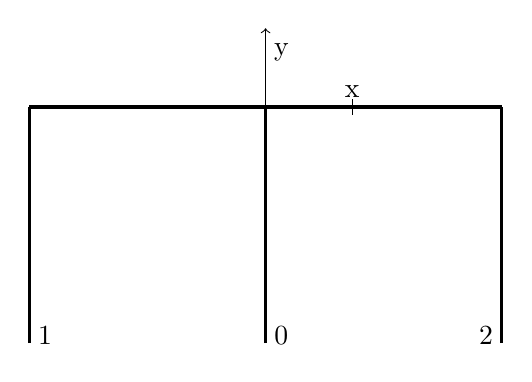
\begin{tikzpicture}
%\draw[thin,dotted] (-3,-3) grid (3,1);
\draw[->] (0,0) -- (0,1);
\node at (0.2,0.7)  {y};
\draw[very thick] (-3,0) -- (3,0);
\draw[very thick] (-3,-3) -- (-3,0);
\draw[very thick] (3,-3) -- (3,0);
\draw[very thick] (0,-3) -- (0,0);
\draw (1.1,-0.1) -- (1.1,0.1);
\node at (1.1,0.2) {x};
\node at (-2.8,-2.9) {1};
\node at (0.2,-2.9) {0};
\node at (2.8,-2.9) {2};
\end{tikzpicture}
\caption{Beam on 3 pillars}
\label {beam3}
\end{figure}
Let the weight of the beam be $W$ and length $2 L$.
Balance of forces gives:
\begin{equation}
        F_0+F_1+F_2=W \label {bf}
\end{equation}
Balance of torques gives:
\begin{equation}
        F_1 L=F_2 L \label {bt}
\end{equation}

   So we have only two equations for three
unknown forces. From the symmetry we can get that $F_1=F_2$. 
(We know that this already from balance of torques.)

{\em First solution}:
All pillars and beam are absolutely rigid. Then
if we pull out the middle pillar nothing will change.
So $F_0=0$ and $F_1=F_2=W/2$.

{\em Second solution}
All pillars and beam are absolutely rigid. Then
we can cat beam at the center and will have two
beams laying on two pillars each.
So $F_0=W/2$ and $F_1=F_2=W/4$.

{\em Third solution}
Beam is absolutely rigid, pillars are very hard springs.
Since beam is horizontal, small change in length is 
equal to all pillars so $F_0=F_1=F_2=w/3$


{\em Fourth solution}
Pillars are rigid, beam is elastic. This case needs
some calculations, well known in elasticity theory
(see e.g \cite {Landau-Lifshitz-7}).
The results is $F_0=5 W/8$ and $F_1=F_2=3 W/16$.

It is clear that all these solutions (and more can be
produced) are limiting cases of standard elasticity 
problem when elasticity coefficients go to infinity.
So generally we can't simply neglect elastic deformations,
we should be more careful.


\section{Units}
\label{units}
Actually to map  physical object into Ideal world of numbers we need some system of units.
What is good about units is that there is plenty of choices.
SI system is the most popular. 
In this system, as described by NIST (National Institute of Standards and Technology, US),
seven base units are defined.
\begin{description}
    \item [time] The second (s) is defined by taking the fixed numerical 
 value of the unperturbed ground-state hyperfine transition 
 frequency of the cesium-133 atom, to be 9,192,631,770 
        when expressed in the unit Hz, which is equal to \unit{ s^{-1}}.
    \item [length] The meter (m) is defined by taking the fixed numerical value of
the speed of light in vacuum c to be 299,792,458 
when expressed in the unit \unit{m.s^{-1}}.
\item [mass] The kilogram (kg) is defined by taking the fixed numerical 
value of the Planck constant h to be $6.62607015 10^{-34}$
when expressed in the unit \unit{J.s}, which is equal to \unit{kg.m^2.s^{-1}}.
\item [electric current] The ampere (A) is defined by taking the fixed numerical value of 
 the elementary charge e to be \num{1.602176634e-19} when expressed in the unit C,
        which is equal to \unit{A.s}.
\item [temperature] The kelvin (K) is defined by taking the fixed numerical value of
    the Boltzmann constant k to be \num{1.380 649e-23} when expressed in the unit \unit{J.K^{-1}}.
\item [amount of substance] Mole (mol) contains exactly \num{6.02214076e23} 
    elementary entities. This number is the fixed numerical value of the Avogadro constant, 
        NA, when expressed in the unit \unit{mol^{-1}}.
\item [luminous intensity] The candela (cd) is defined by taking the fixed numerical 
    value of the luminous efficacy of monochromatic radiation of frequency num{540e12} Hz, Kcd, 
        to be 683 when expressed in the unit \unit{lm.W^{-1}}, which is equal to \unit{cd.sr.W^{-1}}. 
\end{description}
Last three units have no use in theoretical physics and are mentioned for completeness only.

If restricted to length,time and mass all systems of units  differ only 
by scale and hence using of this or that system is a matter of taste. 
For example,to demonstrate good education, one can use 'FFF system' --- Furlong as unit of length (201 m),
Firkin(of water) as unit of mass (41 kg), and Fortnight as unit of time ($ 14\times 86400 s $). 

The situation is more complicated when when we consider electromagnetic phenomena. SI introduces
amper as independent unit which allows to use familiar units for voltage, current and so on.
However the price for that is too high, dimensional permeability of vacuum emerges, components
of electromagnetic field are measured with different units etc. So I shall use Gaussian system,
time is measured in seconds, length in centimeters, and mass in grams. Unit of charge is defined
so that Coulomb low is written as
\[ U= \frac{q_1 q_2}{r} \]
so its dimension is \unit{g^{1/2}.cm^{3/2}.s^{-1}}. 

Anyway, despite of efforts of proponents of SI, a number of external units is popular in practice.
In elementary particle physics energy is mostly measured in electron-volts (\unit{eV}) 
which is equal to  \num{1.602176634e-19} J,
while in
power engineering  in kilowatt-hours (\unit{kW}) equal to \num{3.6e6} J.
Interesting to see that kinetic energy of flying mosquito is approximately 4 \unit{TeV}, and total electric energy 
produced in US in 2022 is approximately \num{1.6e19} J, which correspond to approximately 200 \unit{kg}
according to $ E=m c^2 $ formula.

\section{Numerical methods}
\label{numerical-methods}
TBD

% content of the chapter introduction
\chapter {Introduction}
\label{introduction}
\section{Metaphysics}
\label {metaphysics}
Nature (Real world, Universe) is unique and exists independently of us. The observer who appears in physical
literature is nothing more than figure of speech. `Moon exists even nobody looks at it' and so does electron.
Real word objects behave according to Laws of Nature. Contrary to human laws the Laws of Nature could never be violated.
When we read something like 'this device violates laws of physics' it means usually misunderstanding or clickbait (probably both). Discovering of these laws is the goal of physics. 

To achieve this goal
we build Ideal world and populate it by mathematical models. These models emerge as result of  observations (experiments, measurements, experience), 
their elements appear as ideal images of real objects. Using instruments, 
which may be as simple as measuring tape or lever scaling or as complex as electronic microscope or collider, experimental physics gets facts of Real world.
Theoretical physics constructs and update mathematical models 
on base of these facts.
It should be mentioned that our instruments are part of Real world  and hence described by models\footnote{so a person trying 
to disprove say quantum mechanics would have serious problem since every modern instrument is based actually on quantum 
mechanics.}

    When constructing a model, the following idealization is
   made (see e.g. \cite{Arnold-mt}): 
\begin{itemize}
    \item Events which are  highly probable in Real world become certain in ideal one.
    \item Plausible deductions become proofs.
    \item Some (irrelevant) details disappear.
    \item Approximate results become exact.
\end{itemize}               

This is how abstract notions such as perfectly rigid bodies, incompressible fluids, material points, and so on emerge. 
Even the statement that results of measurement are real numbers is actually idealization: no instrument is able to produce output with infinite number of digits, hence experimental results are always rational numbers.

 When reasonable model is constructed, 
it is investigated and conclusions are mapped back to Real world as predictions which 
should be tested by  experiment. 
If we get  accurate description of reality the model remains {\em reasonable} and can be foundation 
for other models, in particular those describing our instruments, if not it  should be replaced or improved in some way or another.
If the model fails to produce results to be experimentally checked, it simply makes no sense.

Let's assume that we have reasonable (mathematical) model. How can
we obtain correct conclusions from it. 
Purely formal reasoning risks gross errors. 
Particularly dangerous is the temptation to demand precise  definitions for every concept and object in a theory: such definitions often rest on seemingly innocent assumptions 
whose physical meaning is unclear. As a result, one may arrive at impeccably logical conclusions that nonetheless bear no relation to the physical problem at hand.

Here mathematician
and physicist take different paths “The mathematician proves, while the physicist convinces.” \cite{Medvedev}. Mathematician rigorously
and carefully investigates the model as it is formulated.
Physicist may change or abandon the model if it yields 
 incorrect results (contradicting to known experimental facts).
Nature is too complex to be described by one model.
Physicist often uses more than one model simultaneously and change them on the fly 
without warning or use some conditions which were not stated explicitly. 
These tricks irritate mathematicians and confuse engineers. However they are natural parts of 
physicist's way of thinking. 

Contrary to what is said in many (good) books the relations 
among models are not necessary hierarchical. Generally model may be a particular case of another one only in restricted domain. 
For example only system of material points interacting via electromagnetic or (and) gravitational
field constitutes the common subject of classical, relativistic and quantum mechanics and only for such systems classical mechanics may be regarded as special case. Systems with constraints generally can not be described in quantum or relativistic theory.

Formal logic belongs to Ideal world only, on the other hand notions like causality,  likelihood, measurements,
`experimental support' make sense only and in Real world and need 
special care when mapped to Ideal world. 

A lot of paradoxes appear when we mix Real and Ideal world. 
Let us take for example  Hempel's raven paradox: ``observing
of red cow increases the likelihood 
that all ravens are black''. 

Indeed suppose that the statement `All ravens are black' is true.
In the form of an 
implication, this can be expressed as: If something is a raven, then it 
is black. Via contraposition, this statement is equivalent to: If something is 
not black, then it is not a raven. So an observation of, say, red cow supports 
the statement that all ravens are black. This looks very strange but actually is quite
straightforward. In formal logic (Ideal world) there is no such thing as experimental support or
likelihood. Statement may be invalidated by the observation of non black raven, 
but can not be confirmed in any way. So contraposition means simply that the 
statement `raven is found which is not black' is equivalent to 
`something not black is found which is raven'. 

On the other hand common sense (Real world) does not allow statements about 
{\em all} ravens. We should say majority or practically all 
and  contraposition  disappears.

Another good example is Schroedinger's cat. In quantum mechanics the (pure) state of the system is described 
by wave function. Nobody knows exact wave function for an object more complicated than hydrogen atom. 
Surely we can use approximate one, but even in that case preparing of the object in pure state
is rather involved task.  Even if somebody can figure out wave function of cat, how to prepare it
in pure state? May be cool it down to $0^\circ K$? Correlations replace causality in Ideal World.
 Life and death exist in Real World only and have no analogs in Ideal World.

Mathematical problems which required for physical predictions, except in the simplest cases, are so complex that only approximate solutions are possible. 
Often we cannot even verify the validity of the approximations we use,
since this would require exact solutions we cannot obtain. Actually we should 
use some form of perturbation theory ---expansion in series over small parameter(s). 
In most cases the convergence of the series is not proved (and sometimes divergence is proved). 
Another way is numerical approach which of course has its own pitfalls.

\section{Limits are dangerous}
\label{limits}
Limits should be taken with care. A number of theorems describe 
when we can change order of limits and when we can not, how
we can approach to the limit and all that.

Imagine a bucket with small hall at the bottom (in Ideal world),
so we can say that the hole is so small that for all times the bucket remains practically full.
On the other hand we can say that the bucket will be empty if we wait long enough.

Important fact is that two smooth curve may coincide as sets of points, but have
different lengths. Let $ y_n= \sin(n x)/n $ on the  interval $ 0\le x \le 2 \pi $. 
Calculation of length of sinusoidal curve is a simple exercise in elliptic integrals:
\begin{equation}
   \label {sin-length}
   \begin{split}
       l_n=\int_0^{2 \pi}\sqrt{1+\cos^2(nx)}dx\\
       =\int_0^{2 n \pi}\sqrt{1+\cos^2(z)}dz/n\\
       =\int_0^{2 \pi}\sqrt{1+\cos^2(z)}dz\quad \text{does not depend on n}  \\
       =4 \sqrt{2} \int_0^{\pi/2}\sqrt{1-\frac{1}{2} \sin^2(z)}dz\\
       =4 \sqrt{2} E(\frac{1}{\sqrt{2}}) \approx 1.351
   \end{split}
\end{equation}  
and ratio of its length to that of segment is $ \approx 1.22 $ independent of $ n $.
On the other hand maximal distance between the curve and straight segment $ d_n=1/n $ 
vanishes for $ n\rightarrow \infty $.

Contrary to common belief not every properly set problem in
classical mechanics has unique solution. Let's take for example
a (rigid) beam on three (rigid) pillars (see fig.\ref{beam3}).
\begin{figure}[h]
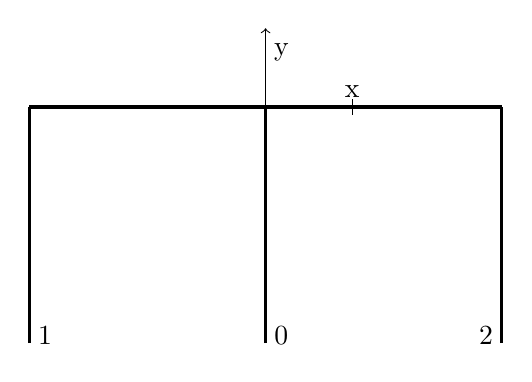
\begin{tikzpicture}
%\draw[thin,dotted] (-3,-3) grid (3,1);
\draw[->] (0,0) -- (0,1);
\node at (0.2,0.7)  {y};
\draw[very thick] (-3,0) -- (3,0);
\draw[very thick] (-3,-3) -- (-3,0);
\draw[very thick] (3,-3) -- (3,0);
\draw[very thick] (0,-3) -- (0,0);
\draw (1.1,-0.1) -- (1.1,0.1);
\node at (1.1,0.2) {x};
\node at (-2.8,-2.9) {1};
\node at (0.2,-2.9) {0};
\node at (2.8,-2.9) {2};
\end{tikzpicture}
\caption{Beam on 3 pillars}
\label {beam3}
\end{figure}
Let the weight of the beam be $W$ and length $2 L$.
Balance of forces gives:
\begin{equation}
        F_0+F_1+F_2=W \label {bf}
\end{equation}
Balance of torques gives:
\begin{equation}
        F_1 L=F_2 L \label {bt}
\end{equation}

   So we have only two equations for three
unknown forces. From the symmetry we can get that $F_1=F_2$. 
(We know that this already from balance of torques.)

{\em First solution}:
All pillars and beam are absolutely rigid. Then
if we pull out the middle pillar nothing will change.
So $F_0=0$ and $F_1=F_2=W/2$.

{\em Second solution}
All pillars and beam are absolutely rigid. Then
we can cat beam at the center and will have two
beams laying on two pillars each.
So $F_0=W/2$ and $F_1=F_2=W/4$.

{\em Third solution}
Beam is absolutely rigid, pillars are very hard springs.
Since beam is horizontal, small change in length is 
equal to all pillars so $F_0=F_1=F_2=w/3$


{\em Fourth solution}
Pillars are rigid, beam is elastic. This case needs
some calculations, well known in elasticity theory
(see e.g \cite {Landau-Lifshitz-7}).
The results is $F_0=5 W/8$ and $F_1=F_2=3 W/16$.

It is clear that all these solutions (and more can be
produced) are limiting cases of standard elasticity 
problem when elasticity coefficients go to infinity.
So generally we can't simply neglect elastic deformations,
we should be more careful.


\section{Units}
\label{units}
Actually to map  physical object into Ideal world of numbers we need some system of units.
What is good about units is that there is plenty of choices.
SI system is the most popular. 
In this system, as described by NIST (National Institute of Standards and Technology, US),
seven base units are defined.
\begin{description}
    \item [time] The second (s) is defined by taking the fixed numerical 
 value of the unperturbed ground-state hyperfine transition 
 frequency of the cesium-133 atom, to be 9,192,631,770 
        when expressed in the unit Hz, which is equal to \unit{ s^{-1}}.
    \item [length] The meter (m) is defined by taking the fixed numerical value of
the speed of light in vacuum c to be 299,792,458 
when expressed in the unit \unit{m.s^{-1}}.
\item [mass] The kilogram (kg) is defined by taking the fixed numerical 
value of the Planck constant h to be $6.62607015 10^{-34}$
when expressed in the unit \unit{J.s}, which is equal to \unit{kg.m^2.s^{-1}}.
\item [electric current] The ampere (A) is defined by taking the fixed numerical value of 
 the elementary charge e to be \num{1.602176634e-19} when expressed in the unit C,
        which is equal to \unit{A.s}.
\item [temperature] The kelvin (K) is defined by taking the fixed numerical value of
    the Boltzmann constant k to be \num{1.380 649e-23} when expressed in the unit \unit{J.K^{-1}}.
\item [amount of substance] Mole (mol) contains exactly \num{6.02214076e23} 
    elementary entities. This number is the fixed numerical value of the Avogadro constant, 
        NA, when expressed in the unit \unit{mol^{-1}}.
\item [luminous intensity] The candela (cd) is defined by taking the fixed numerical 
    value of the luminous efficacy of monochromatic radiation of frequency num{540e12} Hz, Kcd, 
        to be 683 when expressed in the unit \unit{lm.W^{-1}}, which is equal to \unit{cd.sr.W^{-1}}. 
\end{description}
Last three units have no use in theoretical physics and are mentioned for completeness only.

If restricted to length,time and mass all systems of units  differ only 
by scale and hence using of this or that system is a matter of taste. 
For example,to demonstrate good education, one can use 'FFF system' --- Furlong as unit of length (201 m),
Firkin(of water) as unit of mass (41 kg), and Fortnight as unit of time ($ 14\times 86400 s $). 

The situation is more complicated when when we consider electromagnetic phenomena. SI introduces
amper as independent unit which allows to use familiar units for voltage, current and so on.
However the price for that is too high, dimensional permeability of vacuum emerges, components
of electromagnetic field are measured with different units etc. So I shall use Gaussian system,
time is measured in seconds, length in centimeters, and mass in grams. Unit of charge is defined
so that Coulomb low is written as
\[ U= \frac{q_1 q_2}{r} \]
so its dimension is \unit{g^{1/2}.cm^{3/2}.s^{-1}}. 

Anyway, despite of efforts of proponents of SI, a number of external units is popular in practice.
In elementary particle physics energy is mostly measured in electron-volts (\unit{eV}) 
which is equal to  \num{1.602176634e-19} J,
while in
power engineering  in kilowatt-hours (\unit{kW}) equal to \num{3.6e6} J.
Interesting to see that kinetic energy of flying mosquito is approximately 4 \unit{TeV}, and total electric energy 
produced in US in 2022 is approximately \num{1.6e19} J, which correspond to approximately 200 \unit{kg}
according to $ E=m c^2 $ formula.

\section{Numerical methods}
\label{numerical-methods}
TBD


%% contents of the chapter Classical mechanics
\chapter{Classical Mechanics}
\label{class-mech}
{
\setlength\epigraphwidth{0.6\textwidth}
\epigraph {
    Motion\\
There is no motion, said a wise old Greek.\\
The other sage just smiled and walked around.\\
A better answer hardly could be found,\\
And everybody praised this tongue in cheek.\\
But, gentlemen, this funny story might\\
Remind us of a man of great renown:\\
Day after day the Sun walks up and down,\\
And yet the stubborn Galilei was right.
} {A.S. Pushkin, Translated by D. Broytman }
}

One of the most important models in physics is mechanics.
Until the end of the 19th century, mechanics was considered as direct and the only
the basis of all physics. By words understand or
to explain a physical phenomenon meant constructing a mechanical model of it.

Situation has changed,  other physical models exist, e.g. quantum mechanics so 
"usual" mechanics has changed its name to "classical mechanics" and still is
the central part of theoretical physics. All main physical concepts emerged from
it.

As a physical model classical mechanics is based on three principles.
\begin{description}
  \item[ Global Simultaneity] 
    Time is universal and global in classical mechanics. State of the system is determined by
    positions and velocities at fixed time. Every particle has its own coordinates however time
    is common. We can always measure time  exactly and instantly without any influence 
    on mechanical systems. Time is continuous, discrete time would lead to finite difference
    equations instead of differential ones. So dynamics would be undefined, since one always can
    add periodical function to solution.
  \item[ Instant Interaction]
    All interactions are instant i.e. depend on particle states at one and the same moment of time.
    In particular it means that all accelerations and hence evolution is determined by one state (not necessary initial one). It is possible to think that any interaction takes small but finite period of time. This supposition will lead to functional equations instead of differential ones.
  \item [ Precision]
    We can find out and set up exact value of any variable at any time instantly without disturbing
    the system in any way. In particular we can set exactly positions and velocities which means 
    among other things that space is continuous.
\end{description}

There is a great number of books about classical mechanics 
(see e.g\cite{Arnold-cm},\cite{Landau-Lifshitz-1},
\cite{Lanczos},\cite{Goldstein}). 

Let philosophers discuss what is time, space and matter in Real world. 
In Ideal world space is three-dimensional  and euclidean $\mathbb{R}^3$,
mass is real number and time is one-dimensional $\mathbb{T}$.

So universe of classical mechanics is $\mathbb{T} \times \mathbb{R}^3$. 
 The  group of galilean transformations acts on universe \cite{Arnold-cm}. 
Every galilean transformation can be written in a unique way as the composition of a rotation, a translation,
and a uniform motion ($g = g_1 \circ g_2 \circ g_3$), where
\[g_1(t,\vec x)=(t,\vec x+\vec v t)\qquad \forall t\in \mathbb{R},\vec x \in\mathbb{R}^3\] is uniform motion with velocity $\vec v \in\mathbb{R}^3$,
\[g_2(t,\vec x)=(t+t_0,\vec x+\vec x_0)\qquad \forall t\in \mathbb{R},\vec x \in\mathbb{R}^3\] is translation of the origin, and
\[g_3(t,\vec x)=(t,O\vec x)\qquad \forall t\in \mathbb{R},\vec x \in\mathbb{R}^3\] rotation of the coordinate axes ($O:\mathbb{R}^3 \rightarrow \mathbb{R}^3$ is an orthogonal transformation).

Let $M$ be a set. A one-to-one correspondence 
\[\phi_1: M \rightarrow \mathbb{R} \times \mathbb{R}^3\]
is called a galilean (inertial) coordinate system on the set $M$. A coordinate system $\phi_2$ moves
uniformly with respect to $\phi_1$  if $\phi_1\circ\phi_2^{-1}$ is a galilean
transformation. 

Inertial coordinate systems  possess the following two properties:
\begin{enumerate}
    \item All the laws of nature at all moments of time are the same in all inertial coordinate systems;
    \item  All coordinate systems in uniform rectilinear motion with respect to an inertial one are themselves inertial.
\end{enumerate}
This is called `Galileo's principle of relativity'.

The simplest object of classical mechanics is point mass (particle) i.e. object whose shape, 
sizes and internal structure are inessential, so mass (positive scalar $m$) is the only parameter. 
The state of a particle is fully determined by position ($\vec x \in\mathbb{R}^3$) 
and velocity ($\vec v \in\mathbb{R}^3$). 
More accurately: A motion in $\mathbb{R}^n$ is a differentiable mapping 
$\vec x: \mathbb{I}\rightarrow \mathbb{R}^3, \mathbb{I} \subset \mathbb{R}$. 
The derivative $\dot \vec{x}(t_0)=\frac{d\vec x}{dt}|_{t=t_0}$ is called the velocity vector. 
The derivative $\ddot \vec x(t_0)=\frac{ d^2 \vec x}{dt^2}|_{t=t_0}$ is called the acceleration vector. 
The image of motion (curve in $\mathbb{R}^3$) called trajectory and  curve in 
$\mathbb{T} \times \mathbb{R}^3$ which appears  as the graph of a motion, is called a world line.

The initial state of a mechanical system (the totality of positions and
velocities of its points at some moment of time) uniquely determines all of
its motion. In particular, the initial positions and velocities determine the accelerations.
This is called `Newton's principle of determinacy'.

\section{Newtonian mechanics}
\label{newt-mech}

Let us consider the mechanical system consisting of $n$ particles 
with masses $m_j,j=1\ldots n$ and word lines $\vec x_j(t)$.
Suppose that $n$ vector functions  
$\vec F_j:\mathbb{R}^{3 n}\times\mathbb{R}^{3 n}\times\mathbb{R}\rightarrow\mathbb{R}^3,j=1\ldots n$ 
are defined. Then the motion of all particles is determined by equations
\begin{equation}
  \label {newtoneq}
    m_j \ddot \vec x_j=\vec F_j(\vec x_k,\dot \vec x_k,t) \quad j,k=1\ldots n 
\end{equation}
and initial conditions
\begin{equation}
\label {newtonic}
   \vec x_j(t_0)=\vec y_j\quad\dot \vec x_j(t_0)=\vec v_j  \quad j=1\ldots n \end{equation}

Newton's equation \eqref{newtoneq} is  the basis of mechanics. Functions $\vec F_j$
are called forces they should be determined  for each specific mechanical system. If our system
is isolated i.e. includes explicitly all interacting particles, then galilean invariance puts some restrictions on forces.
Namely 
\begin{equation}
  \label {newtoneq-isolated}
    m_j \ddot \vec x_j=\vec F_j(\vec x_j-\vec x_k,\dot \vec x_j-\dot \vec x_k) \quad j,k=1\ldots n 
\end{equation}
practically such systems occur in celestial mechanics. In most other cases the system 
considered is not isolated and forces of general kind \eqref{newtoneq} appear as a result 
of interaction with environment.


Mathematics of  Cauchy problem (\ref{newtoneq},\ref{newtonic}) 
one can find in e.g. \cite{Arnold-ode}. Generally the unique solution exists if
all functions are smooth enough. However smoothness may be violated in physically
important cases, anyway functions $\vec x_j(t)$ should be continuous, $\vec v_j(t)$  may
have finite jumps as a results of strong force acting for very short time (e.g. 
elastic collision).

Note that initial conditions have nothing to do with causality. Causality makes sense in Real world only,
in Ideal world we are free to set final conditions or fix $\vec x_j(t_1)$ and $\vec v_j(t_1)$ for
some intermediate time $t_1$. In many cases we are 
interested in solution of equation \eqref{newtoneq} with fixed initial velocities and final
coordinates  (aiming) or fixed coordinates on both ends (variational problem). Anyway when
conditions are set at two different times  solution may be not unique (unless force is changing relatively slow)
\footnote {I discovered this fact around 1980 and was very proud of myself until I found papers \cite{Maslov-1} and 
\cite{Maslov-2}.}.

        \subsection{Constraints}
In addition to Newton's equations the motion of the system may be restricted by additional equations or inequalities.
Constraints introduce two types of difficulties in the solution of mechanical
problems. First, the coordinates $\vec x_j$ are no longer all independent, since they are
connected by the equations of constraint; hence the equations of motion  
are not all independent. Second, the forces of constraint  are not furnished a priori. 
They are among the unknowns of the problem and must be obtained from the
solution we seek. Indeed, imposing constraints on the system  is simply another
method of stating that there are forces present in the problem that cannot be specified 
directly but are known rather in terms of their effect on the motion of the system.
There is no general method of solving (even numerically) these problems, they are tackled on case by case basis.
To advance we should restrict ourselves with so called holonomic constraints which have the form:
\begin{equation}
        f(\vec x_j,t)=0 \label {hol-const}
\end{equation}

\subsection{Numerical solution}
Generally Newton's equations are to be solved numerically which is a difficult task. 
Two large class of methods are in use:
\begin{enumerate}
        \item "Usual" one-time integrators when differential equations are replaced with finite difference
ones defining snapshots at discrete time steps. These integrators allow accurate description of standard problem:
initial conditions, finite time interval.
\item Geometric integrators which are less accurate for any single trajectory but accurately present qualitative 
        picture for large set of initial data and long times. Such integrators may calculate  coordinates and 
                momenta at different times
\end{enumerate}
One can look for details in \cite{Hairer-Lubich-Wanner} for example. 

\section{Lagrangian mechanics}

If we allow only potential forces i.e. 
\begin{equation}
  \label {potforce}
        \vec F_j(\vec x_k,t)=-\frac{\partial U(\vec x_k,t)}{\partial \vec x_j} \quad j,k=1\ldots n 
\end{equation}
we shall see that equations of motion (\ref{newtoneq}) can be written as 
\begin{equation}
   \label {lagr}
   \begin{split}
      \vec p_j&=\frac{\partial L(\vec x_k,\vec v_k,t)}{\partial \vec v_j} \\ 
        \dot \vec p_j&= \frac{\partial L(\vec x_k,\vec v_k,t)}{\partial \vec x_j}\quad j,k=1\ldots n 
   \end{split}
\end{equation}  
where 
\begin{equation}
  \label{lagr3}
        L(\vec x_k,\vec v_k,t)=\Sigma_1^n \frac{m_k}{2} \vec v_k \cdot \vec v_k-U(\vec x_k,t) 
\end{equation}

If we can solve the equation \[ \vec p_j=\frac{\partial L(\vec x_k,\vec v_k,t)}{\partial \vec v_j} \] for $ \vec v_j $
which of course is not always possible, we can write the equations \eqref{lagr}
in more symmetrical way:
\begin{equation}
   \label {ham}
   \begin{split}
        \dot \vec x_j&=\frac{\partial H(\vec x_k,\vec p_k,t)}{\partial \vec p_j}  \\ 
        \dot \vec p_j&= -\frac{\partial H(\vec x_k,\vec p_k,t)}{\partial \vec x_j}\quad j,k=1\ldots n    
   \end{split}
\end{equation}
where 
\begin{equation}
        H(\vec x_k,\vec p_k,t)=\Sigma_1^n \frac{1}{2 m_k} \vec p_k \cdot \vec p_k+U(\vec x_k,t) \label{ham3}
\end{equation}
Note that functions $L$ (Lagrangian) and $H$ (Hamiltonian) are connected by Legendre transform:
\begin{equation}
        L(\vec x_k,\vec v_k,t)=\Sigma_1^n  \vec p_k \cdot \vec v_k -H(\vec x_k,\vec p_k,t)|_{\vec p_k=m_k\vec v_k}
\quad k=1\ldots n \label {lagr-ham}
\end{equation}


\section{Principle of least action}
\label{least-action}
\begin{definition}
        The equation
        \[\frac{d}{d t}(\frac{\partial L}{\partial \dot x})-\frac{\partial L}{\partial  x}=0 \]
        is called the Euler-Lagrange equation for the functional
        \[\Phi=\int_{t_1}^{t_2} L(x,\dot x,t) dt \]
\end{definition}
Let \( \gamma= \vec x(t) \quad t_1 \le t \le t_2 \) be a curve  in  $\mathbb{R} \times \mathbb{R}^n$ and 
$L: \mathbb{R}^n \times \mathbb{R}^n \times \mathbb{R}\rightarrow \mathbb{R}$ a function of $2 n +1$
variables, then
\begin{theorem}
         The curve $\gamma$ is an extremal of the functional \[\Phi=\int_{t_1}^{t_2} L(\vec x,\dot \vec x,t) dt \]
        on the space of curves joining $(t_1, \vec x_1)$ and $(t_2,\vec x_2)$, if and only if the Euler-
Lagrange equation is satisfied along $\gamma$.
\end{theorem}
This is a system of n second-order equations, and the solution depends on
$2 n$ arbitrary constants. The $2 n$ conditions $x(t_1) = x_0$ and $x(t_2) = x_2$ are used
for finding them.
Two important remarks:
\begin{enumerate}
        \item There may be many extremals connecting two
given points or none at all.
\item The condition for a curve  to be an extremal of a functional does not depend
on the choice of coordinate system. This paves way to geometrisation of mechanics.
\end{enumerate}

It is easy to see that equation of motion (\ref{lagr}) are actually  Euler-Lagrange equations 
for lagrangian \eqref{lagr3}. 
So we have  Hamilton's principle of least action.

I believe that least action principle  is nothing but (powerful) heuristic. Indeed, to compute 
action functional we should define explicitly {\em all} curves connecting given pair of points.
This seems to be impossible or at least very difficult problem. Fortunately we do not need it.
All what we really need is to set configuration space, choose Lagrange function 
\eqref{lagr3} and get equations of motion \eqref{lagr}. It does not matter at all
if we have minimum, maximum, saddle point or whatever property of some functional.

On the other hand having equations of motion as system of ordinary differential equations,
we can transform it into equivalent one, say by multiplying every equation by arbitrary 
function which never becomes zero. This new system may correspond to another Lagrangian and
the difference between new and old one need not come down to total derivative. Most probably
new system will not be Lagrangian at all.

Let us look at simple example --- two-dimensional harmonic oscillator.
Usual Lagrangian is
\begin{equation}
   \label {ho1}
    L_1= \frac{1}{2} (\dot x^2+\dot y^2) -\frac{ \omega^2}{2} ( x^2+ y^2)
\end{equation}
which yields equation  of motions:
\begin{equation}
   \label {hoe1}
   \begin{split}
       \ddot x+ \omega^2 x & =0 \\
       \ddot y+ \omega^2 y & =0 
   \end{split}
\end{equation}
Same equations of motion come form 
another Lagrangian
\begin{equation}
   \label {ho2}
    L_2= \frac{1}{2} (\dot x^2-\dot y^2) -\frac{ \omega^2}{2} ( x^2- y^2)
\end{equation}
or
\begin{equation}
   \label {ho3}
    L_3= \dot x\dot y - \omega^2  x y
\end{equation}
corresponding  Hamiltonians 
\begin{equation}
   \label {ho2h}
    H_2= \frac{1}{2} ( p_x^2-p_y^2) +\frac{ \omega^2}{2} ( x^2- y^2)
\end{equation}
and
\begin{equation}
   \label {ho3h}
    H_3= p_x p_y +\omega^2  x y
\end{equation}
are not even positive definite!

\section{Gauge invariance} 
\label{gauge-invariance}

From now on we shall use generalized coordinates $ q=\{q_j, j=1\ldots n\} $, where $ n $ is the number of
degrees of freedom. These coordinates may have or have not physical meaning.

We are used to think that gauge invariance is about electromagnetism, actually it appears
already in classical mechanics. It is easy to prove that adding the total derivative
\begin{equation}
   \label {tot-der}
    \frac{d \Phi (q,t)}{d t}=\frac{\partial \Phi(q,t)}{\partial t} + \frac{ \partial \Phi (q,t)}{\partial q_j} \dot q_j
\end{equation}
to Lagrangian does not change equations of motion. However canonical momenta
\begin{equation}
   \label {can-mom}
   p_j=\frac{ \partial L(q,\dot q,t)}{\partial \dot q_j}
\end{equation}

becomes \[ P_j=p_j+\frac{\partial \Phi}{\partial q_j} \] Transformation $ p,q \rightarrow P,q $ is evidently
canonical and new Hamiltonian becomes 
\[ H_{new}=H(p(P),q)- \frac{\partial \Phi}{\partial t}\]
The fact that canonical momenta have no physical meaning is not a weak but strong point of Hamiltonian 
mechanics.

I skip the  discussion of standard things like Poisson brackets, integrals of motion and all that.

\section{"Spin" in constant magnetic field}
\label{mag-mom}
We used to natural systems where hamiltonian is quadratic form over momenta,
but there are physical systems with hamiltonians linear over momenta.
So lagrangian does not exist. Let us consider 
dynamic of point magnetic moment in constant magnetic field has not only
clear physical meaning but also significant practical value. I investigated
this problem (actually slightly more general one) in connection with control of MRI
scanner \cite{RPZ4},\cite{RPZ3},\cite{RPZ2},\cite{RPZ1}.


Hamiltonian is $ H=\vec M \cdot \vec B $ where $\vec M$ is magnetic moment 
and $ \vec B $ is constant magnetic field.
It is convenient to write $ \vec M=\frac{e}{m c}\vec S $ where $ \vec S $
is angular moment ("spin")  and  include gyromagnetic ratio into magnetic field
$ \vec \Omega = \frac{e}{m c}\vec B$. Components of $ \vec S $ are not
canonical variables, their Poisson brackets are
\begin{equation}
   \label {pb}
    \{S_i,S_j\}= \epsilon_{ijk} S_k
\end{equation}
However they define phase space (sphere)  and equation of motion:
\begin{equation}
   \label {sp1}
    \dot S_i=\{S_i,H\}
\end{equation} 
or 
\begin{equation}
   \label {sp2}
    \dot {\vec S} =-\vec S \times \vec \Omega
\end{equation}

In canonical variables 
\begin{equation}
   \label {sp3}
   \begin{split}
       S_x & = \sqrt{S^2-p^2} \cos q \\
       S_y & = \sqrt{S^2-p^2} \sin q \\
       S_z & = p,\quad -S\le p \le S
   \end{split}
\end{equation}
Let $ \vec \Omega =(0,0, \Omega) $ then $ H=p \Omega $ and canonical equations are:
\begin{equation}
   \label {sp4}
   \begin{split}
       \dot p & =0\\
       \dot q & = \Omega
   \end{split}
\end{equation}
Lagrangian $ L=0 $, so we can not get equations of motion as second order equation.

Moment $ p $ is integral of motion which is fine but velocity is not connected to 
moment at all, it is constant. For pair of points in phase space generally there is
no trajectory passable for given time. Variation problem simply can not be posed.

 Hamiltonian $ H=p \Omega $ looks like that for harmonic oscillator in action-angle variables
and so we can  transform it to usual quadratic form, but the condition $  -S\le p \le S$
makes this transformation pure formal.

% contents of the chapter Classical mechanics
\chapter{Classical Mechanics}
\label{class-mech}
{
\setlength\epigraphwidth{0.6\textwidth}
\epigraph {
    Motion\\
There is no motion, said a wise old Greek.\\
The other sage just smiled and walked around.\\
A better answer hardly could be found,\\
And everybody praised this tongue in cheek.\\
But, gentlemen, this funny story might\\
Remind us of a man of great renown:\\
Day after day the Sun walks up and down,\\
And yet the stubborn Galilei was right.
} {A.S. Pushkin, Translated by D. Broytman }
}

One of the most important models in physics is mechanics.
Until the end of the 19th century, mechanics was considered as direct and the only
the basis of all physics. By words understand or
to explain a physical phenomenon meant constructing a mechanical model of it.

Situation has changed,  other physical models exist, e.g. quantum mechanics so 
"usual" mechanics has changed its name to "classical mechanics" and still is
the central part of theoretical physics. All main physical concepts emerged from
it.

As a physical model classical mechanics is based on three principles.
\begin{description}
  \item[ Global Simultaneity] 
    Time is universal and global in classical mechanics. State of the system is determined by
    positions and velocities at fixed time. Every particle has its own coordinates however time
    is common. We can always measure time  exactly and instantly without any influence 
    on mechanical systems. Time is continuous, discrete time would lead to finite difference
    equations instead of differential ones. So dynamics would be undefined, since one always can
    add periodical function to solution.
  \item[ Instant Interaction]
    All interactions are instant i.e. depend on particle states at one and the same moment of time.
    In particular it means that all accelerations and hence evolution is determined by one state (not necessary initial one). It is possible to think that any interaction takes small but finite period of time. This supposition will lead to functional equations instead of differential ones.
  \item [ Precision]
    We can find out and set up exact value of any variable at any time instantly without disturbing
    the system in any way. In particular we can set exactly positions and velocities which means 
    among other things that space is continuous.
\end{description}

There is a great number of books about classical mechanics 
(see e.g\cite{Arnold-cm},\cite{Landau-Lifshitz-1},
\cite{Lanczos},\cite{Goldstein}). 

Let philosophers discuss what is time, space and matter in Real world. 
In Ideal world space is three-dimensional  and euclidean $\mathbb{R}^3$,
mass is real number and time is one-dimensional $\mathbb{T}$.

So universe of classical mechanics is $\mathbb{T} \times \mathbb{R}^3$. 
 The  group of galilean transformations acts on universe \cite{Arnold-cm}. 
Every galilean transformation can be written in a unique way as the composition of a rotation, a translation,
and a uniform motion ($g = g_1 \circ g_2 \circ g_3$), where
\[g_1(t,\vec x)=(t,\vec x+\vec v t)\qquad \forall t\in \mathbb{R},\vec x \in\mathbb{R}^3\] is uniform motion with velocity $\vec v \in\mathbb{R}^3$,
\[g_2(t,\vec x)=(t+t_0,\vec x+\vec x_0)\qquad \forall t\in \mathbb{R},\vec x \in\mathbb{R}^3\] is translation of the origin, and
\[g_3(t,\vec x)=(t,O\vec x)\qquad \forall t\in \mathbb{R},\vec x \in\mathbb{R}^3\] rotation of the coordinate axes ($O:\mathbb{R}^3 \rightarrow \mathbb{R}^3$ is an orthogonal transformation).

Let $M$ be a set. A one-to-one correspondence 
\[\phi_1: M \rightarrow \mathbb{R} \times \mathbb{R}^3\]
is called a galilean (inertial) coordinate system on the set $M$. A coordinate system $\phi_2$ moves
uniformly with respect to $\phi_1$  if $\phi_1\circ\phi_2^{-1}$ is a galilean
transformation. 

Inertial coordinate systems  possess the following two properties:
\begin{enumerate}
    \item All the laws of nature at all moments of time are the same in all inertial coordinate systems;
    \item  All coordinate systems in uniform rectilinear motion with respect to an inertial one are themselves inertial.
\end{enumerate}
This is called `Galileo's principle of relativity'.

The simplest object of classical mechanics is point mass (particle) i.e. object whose shape, 
sizes and internal structure are inessential, so mass (positive scalar $m$) is the only parameter. 
The state of a particle is fully determined by position ($\vec x \in\mathbb{R}^3$) 
and velocity ($\vec v \in\mathbb{R}^3$). 
More accurately: A motion in $\mathbb{R}^n$ is a differentiable mapping 
$\vec x: \mathbb{I}\rightarrow \mathbb{R}^3, \mathbb{I} \subset \mathbb{R}$. 
The derivative $\dot \vec{x}(t_0)=\frac{d\vec x}{dt}|_{t=t_0}$ is called the velocity vector. 
The derivative $\ddot \vec x(t_0)=\frac{ d^2 \vec x}{dt^2}|_{t=t_0}$ is called the acceleration vector. 
The image of motion (curve in $\mathbb{R}^3$) called trajectory and  curve in 
$\mathbb{T} \times \mathbb{R}^3$ which appears  as the graph of a motion, is called a world line.

The initial state of a mechanical system (the totality of positions and
velocities of its points at some moment of time) uniquely determines all of
its motion. In particular, the initial positions and velocities determine the accelerations.
This is called `Newton's principle of determinacy'.

\section{Newtonian mechanics}
\label{newt-mech}

Let us consider the mechanical system consisting of $n$ particles 
with masses $m_j,j=1\ldots n$ and word lines $\vec x_j(t)$.
Suppose that $n$ vector functions  
$\vec F_j:\mathbb{R}^{3 n}\times\mathbb{R}^{3 n}\times\mathbb{R}\rightarrow\mathbb{R}^3,j=1\ldots n$ 
are defined. Then the motion of all particles is determined by equations
\begin{equation}
  \label {newtoneq}
    m_j \ddot \vec x_j=\vec F_j(\vec x_k,\dot \vec x_k,t) \quad j,k=1\ldots n 
\end{equation}
and initial conditions
\begin{equation}
\label {newtonic}
   \vec x_j(t_0)=\vec y_j\quad\dot \vec x_j(t_0)=\vec v_j  \quad j=1\ldots n \end{equation}

Newton's equation \eqref{newtoneq} is  the basis of mechanics. Functions $\vec F_j$
are called forces they should be determined  for each specific mechanical system. If our system
is isolated i.e. includes explicitly all interacting particles, then galilean invariance puts some restrictions on forces.
Namely 
\begin{equation}
  \label {newtoneq-isolated}
    m_j \ddot \vec x_j=\vec F_j(\vec x_j-\vec x_k,\dot \vec x_j-\dot \vec x_k) \quad j,k=1\ldots n 
\end{equation}
practically such systems occur in celestial mechanics. In most other cases the system 
considered is not isolated and forces of general kind \eqref{newtoneq} appear as a result 
of interaction with environment.


Mathematics of  Cauchy problem (\ref{newtoneq},\ref{newtonic}) 
one can find in e.g. \cite{Arnold-ode}. Generally the unique solution exists if
all functions are smooth enough. However smoothness may be violated in physically
important cases, anyway functions $\vec x_j(t)$ should be continuous, $\vec v_j(t)$  may
have finite jumps as a results of strong force acting for very short time (e.g. 
elastic collision).

Note that initial conditions have nothing to do with causality. Causality makes sense in Real world only,
in Ideal world we are free to set final conditions or fix $\vec x_j(t_1)$ and $\vec v_j(t_1)$ for
some intermediate time $t_1$. In many cases we are 
interested in solution of equation \eqref{newtoneq} with fixed initial velocities and final
coordinates  (aiming) or fixed coordinates on both ends (variational problem). Anyway when
conditions are set at two different times  solution may be not unique (unless force is changing relatively slow)
\footnote {I discovered this fact around 1980 and was very proud of myself until I found papers \cite{Maslov-1} and 
\cite{Maslov-2}.}.

        \subsection{Constraints}
In addition to Newton's equations the motion of the system may be restricted by additional equations or inequalities.
Constraints introduce two types of difficulties in the solution of mechanical
problems. First, the coordinates $\vec x_j$ are no longer all independent, since they are
connected by the equations of constraint; hence the equations of motion  
are not all independent. Second, the forces of constraint  are not furnished a priori. 
They are among the unknowns of the problem and must be obtained from the
solution we seek. Indeed, imposing constraints on the system  is simply another
method of stating that there are forces present in the problem that cannot be specified 
directly but are known rather in terms of their effect on the motion of the system.
There is no general method of solving (even numerically) these problems, they are tackled on case by case basis.
To advance we should restrict ourselves with so called holonomic constraints which have the form:
\begin{equation}
        f(\vec x_j,t)=0 \label {hol-const}
\end{equation}

\subsection{Numerical solution}
Generally Newton's equations are to be solved numerically which is a difficult task. 
Two large class of methods are in use:
\begin{enumerate}
        \item "Usual" one-time integrators when differential equations are replaced with finite difference
ones defining snapshots at discrete time steps. These integrators allow accurate description of standard problem:
initial conditions, finite time interval.
\item Geometric integrators which are less accurate for any single trajectory but accurately present qualitative 
        picture for large set of initial data and long times. Such integrators may calculate  coordinates and 
                momenta at different times
\end{enumerate}
One can look for details in \cite{Hairer-Lubich-Wanner} for example. 

\section{Lagrangian mechanics}

If we allow only potential forces i.e. 
\begin{equation}
  \label {potforce}
        \vec F_j(\vec x_k,t)=-\frac{\partial U(\vec x_k,t)}{\partial \vec x_j} \quad j,k=1\ldots n 
\end{equation}
we shall see that equations of motion (\ref{newtoneq}) can be written as 
\begin{equation}
   \label {lagr}
   \begin{split}
      \vec p_j&=\frac{\partial L(\vec x_k,\vec v_k,t)}{\partial \vec v_j} \\ 
        \dot \vec p_j&= \frac{\partial L(\vec x_k,\vec v_k,t)}{\partial \vec x_j}\quad j,k=1\ldots n 
   \end{split}
\end{equation}  
where 
\begin{equation}
  \label{lagr3}
        L(\vec x_k,\vec v_k,t)=\Sigma_1^n \frac{m_k}{2} \vec v_k \cdot \vec v_k-U(\vec x_k,t) 
\end{equation}

If we can solve the equation \[ \vec p_j=\frac{\partial L(\vec x_k,\vec v_k,t)}{\partial \vec v_j} \] for $ \vec v_j $
which of course is not always possible, we can write the equations \eqref{lagr}
in more symmetrical way:
\begin{equation}
   \label {ham}
   \begin{split}
        \dot \vec x_j&=\frac{\partial H(\vec x_k,\vec p_k,t)}{\partial \vec p_j}  \\ 
        \dot \vec p_j&= -\frac{\partial H(\vec x_k,\vec p_k,t)}{\partial \vec x_j}\quad j,k=1\ldots n    
   \end{split}
\end{equation}
where 
\begin{equation}
        H(\vec x_k,\vec p_k,t)=\Sigma_1^n \frac{1}{2 m_k} \vec p_k \cdot \vec p_k+U(\vec x_k,t) \label{ham3}
\end{equation}
Note that functions $L$ (Lagrangian) and $H$ (Hamiltonian) are connected by Legendre transform:
\begin{equation}
        L(\vec x_k,\vec v_k,t)=\Sigma_1^n  \vec p_k \cdot \vec v_k -H(\vec x_k,\vec p_k,t)|_{\vec p_k=m_k\vec v_k}
\quad k=1\ldots n \label {lagr-ham}
\end{equation}


\section{Principle of least action}
\label{least-action}
\begin{definition}
        The equation
        \[\frac{d}{d t}(\frac{\partial L}{\partial \dot x})-\frac{\partial L}{\partial  x}=0 \]
        is called the Euler-Lagrange equation for the functional
        \[\Phi=\int_{t_1}^{t_2} L(x,\dot x,t) dt \]
\end{definition}
Let \( \gamma= \vec x(t) \quad t_1 \le t \le t_2 \) be a curve  in  $\mathbb{R} \times \mathbb{R}^n$ and 
$L: \mathbb{R}^n \times \mathbb{R}^n \times \mathbb{R}\rightarrow \mathbb{R}$ a function of $2 n +1$
variables, then
\begin{theorem}
         The curve $\gamma$ is an extremal of the functional \[\Phi=\int_{t_1}^{t_2} L(\vec x,\dot \vec x,t) dt \]
        on the space of curves joining $(t_1, \vec x_1)$ and $(t_2,\vec x_2)$, if and only if the Euler-
Lagrange equation is satisfied along $\gamma$.
\end{theorem}
This is a system of n second-order equations, and the solution depends on
$2 n$ arbitrary constants. The $2 n$ conditions $x(t_1) = x_0$ and $x(t_2) = x_2$ are used
for finding them.
Two important remarks:
\begin{enumerate}
        \item There may be many extremals connecting two
given points or none at all.
\item The condition for a curve  to be an extremal of a functional does not depend
on the choice of coordinate system. This paves way to geometrisation of mechanics.
\end{enumerate}

It is easy to see that equation of motion (\ref{lagr}) are actually  Euler-Lagrange equations 
for lagrangian \eqref{lagr3}. 
So we have  Hamilton's principle of least action.

I believe that least action principle  is nothing but (powerful) heuristic. Indeed, to compute 
action functional we should define explicitly {\em all} curves connecting given pair of points.
This seems to be impossible or at least very difficult problem. Fortunately we do not need it.
All what we really need is to set configuration space, choose Lagrange function 
\eqref{lagr3} and get equations of motion \eqref{lagr}. It does not matter at all
if we have minimum, maximum, saddle point or whatever property of some functional.

On the other hand having equations of motion as system of ordinary differential equations,
we can transform it into equivalent one, say by multiplying every equation by arbitrary 
function which never becomes zero. This new system may correspond to another Lagrangian and
the difference between new and old one need not come down to total derivative. Most probably
new system will not be Lagrangian at all.

Let us look at simple example --- two-dimensional harmonic oscillator.
Usual Lagrangian is
\begin{equation}
   \label {ho1}
    L_1= \frac{1}{2} (\dot x^2+\dot y^2) -\frac{ \omega^2}{2} ( x^2+ y^2)
\end{equation}
which yields equation  of motions:
\begin{equation}
   \label {hoe1}
   \begin{split}
       \ddot x+ \omega^2 x & =0 \\
       \ddot y+ \omega^2 y & =0 
   \end{split}
\end{equation}
Same equations of motion come form 
another Lagrangian
\begin{equation}
   \label {ho2}
    L_2= \frac{1}{2} (\dot x^2-\dot y^2) -\frac{ \omega^2}{2} ( x^2- y^2)
\end{equation}
or
\begin{equation}
   \label {ho3}
    L_3= \dot x\dot y - \omega^2  x y
\end{equation}
corresponding  Hamiltonians 
\begin{equation}
   \label {ho2h}
    H_2= \frac{1}{2} ( p_x^2-p_y^2) +\frac{ \omega^2}{2} ( x^2- y^2)
\end{equation}
and
\begin{equation}
   \label {ho3h}
    H_3= p_x p_y +\omega^2  x y
\end{equation}
are not even positive definite!

\section{Gauge invariance} 
\label{gauge-invariance}

From now on we shall use generalized coordinates $ q=\{q_j, j=1\ldots n\} $, where $ n $ is the number of
degrees of freedom. These coordinates may have or have not physical meaning.

We are used to think that gauge invariance is about electromagnetism, actually it appears
already in classical mechanics. It is easy to prove that adding the total derivative
\begin{equation}
   \label {tot-der}
    \frac{d \Phi (q,t)}{d t}=\frac{\partial \Phi(q,t)}{\partial t} + \frac{ \partial \Phi (q,t)}{\partial q_j} \dot q_j
\end{equation}
to Lagrangian does not change equations of motion. However canonical momenta
\begin{equation}
   \label {can-mom}
   p_j=\frac{ \partial L(q,\dot q,t)}{\partial \dot q_j}
\end{equation}

becomes \[ P_j=p_j+\frac{\partial \Phi}{\partial q_j} \] Transformation $ p,q \rightarrow P,q $ is evidently
canonical and new Hamiltonian becomes 
\[ H_{new}=H(p(P),q)- \frac{\partial \Phi}{\partial t}\]
The fact that canonical momenta have no physical meaning is not a weak but strong point of Hamiltonian 
mechanics.

I skip the  discussion of standard things like Poisson brackets, integrals of motion and all that.

\section{"Spin" in constant magnetic field}
\label{mag-mom}
We used to natural systems where hamiltonian is quadratic form over momenta,
but there are physical systems with hamiltonians linear over momenta.
So lagrangian does not exist. Let us consider 
dynamic of point magnetic moment in constant magnetic field has not only
clear physical meaning but also significant practical value. I investigated
this problem (actually slightly more general one) in connection with control of MRI
scanner \cite{RPZ4},\cite{RPZ3},\cite{RPZ2},\cite{RPZ1}.


Hamiltonian is $ H=\vec M \cdot \vec B $ where $\vec M$ is magnetic moment 
and $ \vec B $ is constant magnetic field.
It is convenient to write $ \vec M=\frac{e}{m c}\vec S $ where $ \vec S $
is angular moment ("spin")  and  include gyromagnetic ratio into magnetic field
$ \vec \Omega = \frac{e}{m c}\vec B$. Components of $ \vec S $ are not
canonical variables, their Poisson brackets are
\begin{equation}
   \label {pb}
    \{S_i,S_j\}= \epsilon_{ijk} S_k
\end{equation}
However they define phase space (sphere)  and equation of motion:
\begin{equation}
   \label {sp1}
    \dot S_i=\{S_i,H\}
\end{equation} 
or 
\begin{equation}
   \label {sp2}
    \dot {\vec S} =-\vec S \times \vec \Omega
\end{equation}

In canonical variables 
\begin{equation}
   \label {sp3}
   \begin{split}
       S_x & = \sqrt{S^2-p^2} \cos q \\
       S_y & = \sqrt{S^2-p^2} \sin q \\
       S_z & = p,\quad -S\le p \le S
   \end{split}
\end{equation}
Let $ \vec \Omega =(0,0, \Omega) $ then $ H=p \Omega $ and canonical equations are:
\begin{equation}
   \label {sp4}
   \begin{split}
       \dot p & =0\\
       \dot q & = \Omega
   \end{split}
\end{equation}
Lagrangian $ L=0 $, so we can not get equations of motion as second order equation.

Moment $ p $ is integral of motion which is fine but velocity is not connected to 
moment at all, it is constant. For pair of points in phase space generally there is
no trajectory passable for given time. Variation problem simply can not be posed.

 Hamiltonian $ H=p \Omega $ looks like that for harmonic oscillator in action-angle variables
and so we can  transform it to usual quadratic form, but the condition $  -S\le p \le S$
makes this transformation pure formal.


%%content of the chapter classical electrodynamics
\chapter{Classical Electrodynamics}
\label{class-ed}
\section{Microscopic Maxwell Equations}
\label{micro-maxwell-eqs}

Omitting the long history of misconceptions and discoveries, 
one may say that, in addition to mass, particles may possess 
electric charge. Like mass, it is a scalar quantity, but unlike mass, 
charge may be positive, negative, or zero.
To describe the interaction of charged particles, 
it is necessary to introduce a new entity --- the electromagnetic field $ (\vec E(\vec r,t),\vec B(\vec r,t)) $.

The motion of  particle with charge $ e $ is described by Lorentz force
\begin{equation}
   \label {lorentz-force}
   \frac{d \vec p}{d t}=e \vec E(\vec r,t) + \frac{e}{c}\vec v \times \vec B(\vec r,t)
\end{equation}
Dynamics of electromagnetic field is described   Maxwell’s equations:
\begin{align}
\nabla \times \vec{E} + \frac{1}{c}\frac{\partial \vec{B}}{\partial t} &= 0, \label{me-faraday} \\
\nabla \cdot \vec{B} &= 0, \label{me-monopole} \\
\nabla \cdot \vec{E} &= 4\pi \rho, \label{me-gauss} \\
\nabla \times \vec{B} - \frac{1}{c}\frac{\partial \vec{E}}{\partial t} &= \frac{4\pi}{c}\vec{j}. \label{me-ampere}
\end{align}
Here 
\begin{equation}
   \label {dens1}
    \rho(\vec r,t)=\Sigma_a e_a \delta (\vec r-\vec r_a)
\end{equation}
and
\begin{equation}
   \label {curr1}
    \vec j(\vec r,t)=\Sigma_a e_a \vec v_a \delta (\vec r-\vec r_a)
\end{equation}
It is important to know that $ \delta $-function is actually not a function, but distribution
--- linear functional on the space of test functions. It is very useful in linear problems
but makes a lot of troubles in non-linear ones.

Taking the divergence of \eqref{me-ampere} and using \eqref{me-gauss} yields the continuity equation:
\begin{equation}
    \label{cont}
\partial_t \rho + \nabla \cdot \vec{j} = 0,
\end{equation}
demonstrating that charge conservation is not an independent 
postulate but a structural consequence of Maxwell’s equations.
In particular \eqref{dens1} and \eqref{curr1} satisfy \eqref{cont}.

\section{Maxwell Equations in Media}
\label{maxwell-eqs}


In media we can somehow divide charges and currents into two groups: 
bound ones which belong to media and free ones.
Bound charges can be expressed as
\begin{equation}
   \label {bound-charge}
   \rho_b=-\nabla \vec P
\end{equation}
where $ \vec P $  (polarization) is the dipole moment of unit volume
\begin{equation}
   \label {bound-current}
   \vec j_b =\frac{\partial \vec P}{\partial t}+ c \nabla \times \vec M
\end{equation}
where $ \vec M$ (magnetization) is the magnetic dipole moment of unit volume.

Thus macroscopic (averaged) charge and current densities become
\begin{equation}
   \label {tot-cur-ch}
   \vec j=\vec j_f+ \vec j_b \qquad \rho=\rho_f+\rho_b
\end{equation}
and macroscopic Maxwell equations read:
\begin{align}
    \nabla \cdot \vec{E} &= 4\pi (\rho_f -\nabla \vec P), \label{me-g1} \\
    \nabla \times \vec{B} - \frac{1}{c}\frac{\partial \vec{E}}{\partial t} &= 
    \frac{4\pi}{c}(\vec j_f+\frac{\partial \vec P}{\partial t}+ c \nabla \times \vec M). \label{me-a1}
\end{align}
or:
\begin{align}
    \nabla \cdot \vec D &= 4\pi \rho_f , \label{me-g2} \\
    \nabla \times \vec H - \frac{1}{c}\frac{\partial \vec D}{\partial t} &= \frac{4\pi}{c}\vec j_f . \label{me-a2}
\end{align}
Here $ \vec D = \vec E+4 \pi \vec P $ and $ \vec H = \vec E-4 \pi \vec M $.
In equations \eqref{me-g2} and \eqref{me-a2} $ \rho $ and $ \vec j $ are supposed to be smooth
functions as a result of averaging of \eqref{dens1} and \eqref{curr1}.
Homogeneous equations \eqref{me-faraday} and \eqref{me-monopole} remain the same.  

Some information about media should be added to make Maxwell
equations solvable. Usually it is done by introducing constitutive
relations and generalized Ohm's law which define somehow 
$ \vec H $ , $ \vec D $ and $ \vec j $ in terms of 
$ \vec E $ and $ \vec B $. A lot of interesting physics
is contained in specific form of these relations.

\section{Gauge Transformations}
\label{gauge-transformations}

It is convenient to introduce scalar $\phi$ and vector $\vec A$ such that
\begin{equation}
   \label {potA}
   \vec B = \nabla \times \vec A \quad \vec E = -\frac{1}{c} \frac{\partial \vec A}{\partial t} - \nabla \phi
\end{equation}
so the equations \eqref{me-monopole} and \eqref{me-faraday} become identities, remaining equations will
take the form
\begin{equation}
   \label {me-pot}
   \begin{split}
       \Box \vec A + \nabla ( \nabla \cdot \vec A+ \frac{1}{c} \dot \phi) &= \frac{4 \pi}{c} \vec j \\
       \Box \phi -\frac{1}{c} \frac{\partial}{\partial t}( \nabla \cdot \vec A+ \frac{1}{c} \dot \phi) & = 4 \pi \rho
   \end{split}
\end{equation}
Here $ \Box $ is d'alambert operator defined as \[  \frac{1}{c^2} \frac{\partial^2}{\partial t^2}-\nabla^2 \]

Equations \eqref{potA} do not define potentials uniquely, gauge transformation: 
\begin{equation}
   \label {gauge-transformation}
   \begin{split}
       \vec A &\rightarrow \vec A+ \nabla \chi \\
       \phi & \rightarrow \phi - \dot \chi /c
   \end{split}
\end{equation}
 where $ \chi  $ is arbitrary leaves fields $ \vec B $
and $ \vec E $ unchanged. So we can prescribe additional
condition (gauge) on potentials.

If we prescribe the condition :
\begin{equation}
   \label {lg}
    \nabla \cdot \vec A+ \frac{1}{c} \dot \phi=0
\end{equation}
which is evidently compatible with \eqref{cont} equations \eqref{me-pot} separate and read:
\begin{equation}
   \label {me-pot-lg}
   \begin{split}
       \Box \vec A &= -\frac{4 \pi}{c} \vec j \\
       \Box \phi  & = -4 \pi \rho
   \end{split}
\end{equation}


The Lorenz gauge \eqref{lg} is the most popular one, it
allows us to uncouple equations \eqref{me-pot-lg}   so that the scalar and vector
potentials are described by symmetrical uncoupled wave equations,
which is a characteristic of this gauge. 
%It is the only covariant gauge.
However even Lorenz condition leaves some arbitrariness: $ \chi \rightarrow \chi + \psi $ 
 in \eqref{gauge-transformation} changes nothing if $ \Box \psi=0 $.

A less popular gauge in textbooks is the Coulomb gauge.
\begin{equation}
   \label {cg}
   \nabla \cdot \vec A=0
\end{equation}
In this gauge the scalar potential satisfies an instantaneous
Poisson equation, which is a peculiar characteristic of this
gauge.
A number of other gauges was studied in \cite{heras}:
Kirchhoff gauge:
\begin{equation}
   \label {kg}
    \nabla \cdot \vec A- \frac{1}{c} \dot \phi=0
\end{equation}
which can be seen as Lorenz gauge in Euclidean 4-space.
Velocity gauge:
\begin{equation}
   \label {vg}
    \nabla \cdot \vec A- \frac{1}{v} \dot \phi=0
\end{equation}
The velocity gauge is one in which the scalar
potential propagates with an arbitrary speed. This gauge is
not well known despite the fact that it was proposed several
years ago. The v-gauge is really a family of gauges that
contains the Lorenz and Coulomb gauges as particular cases
and also includes the Kirchhoff gauge.

Temporal gauge:
\begin{equation}
   \label {tg}
   \phi=0
\end{equation}
 The temporal gauge is one in which 
the scalar potential is identically zero, which means that 
the electric and magnetic fields are defined 
only by the vector potential.

It is shown in \cite{heras} that  all these  potentials yield the 
same  retarded
electric and magnetic fields. 

\section {Covariant Form of Maxwell Equations}
\label{me-cov}

Introducing (formally) fourth coordinate $ x^0=c t $ we can define
 Minkowski space as  the manifold $M \cong \mathbb{R}^4$ 
equipped with the  metric
\begin{equation}
   \label {minkg}
    g_{i j} = g^{i j}=\mathrm{diag}(1,-1,-1,-1).
\end{equation} 
The meaning of it will be discussed later, meanwhile
it is used only to simplify notations. So
\begin{align}
    x^i&=(ct,\vec x) \label{x4} \\
    A^i&=(\phi,\vec A) \label{a4}\\
    j^i&=(c \rho, \vec j) \label{j4}\\
    \partial_i&= \frac{\partial}{\partial x^i} \label{d4}
\end{align}
So $ \Box=g^{i k} \partial_i \partial_k $ 
Lorenz gauge \eqref{lg} reads:
\begin{equation}
   \label {lgc}
   \partial_i A^i=0
\end{equation} 
 continuity equation \eqref{cont} becomes
\begin{equation}
   \label {contc}
   \partial_i j^i=0
\end{equation} 
and Maxwell equations \eqref{me-pot} take the form:
\begin{equation}
   \label {me-potc}
    \Box A^i= \frac{4 \pi}{c} j^i
\end{equation}

The fields $ (\vec E,\vec B) $ in covariant formalism
become parts of antisymmetric tensor of second rank:
\begin{equation}
   \label {ebc}
    F_{i k}=\partial_i A_k-\partial_k A_i
\end{equation}
where $ A_k=g_{k i} A^i=(\phi,-\vec A) $ so equations \eqref{me-gauss}
and \eqref{me-ampere} take the form
\begin{equation}
   \label {mec}
    \partial_k F^{i k}=-\frac{4 \pi}{c} j^k
\end{equation}

One can easily see that Maxwell equations save their form
under linear transformations preserving metric \eqref{minkg}.
However Galilean transformations change them, in particular
the velocity of light does not depend on inertial frame of
reference, which contradicts the rule of adding velocities.


It is often stated that the fields $ (\vec E,\vec B) $ or
$ F_{i k} $ are the physical variables and potentials
$A^i$ have no physical meaning. This statement based
on fact that potentials $ A^i $ are not gauge invariant.
However with argument is not sound, following this logic
we must declare canonical momenta as not physical since
it  is also not gauge invariant (see section \ref{gauge-invariance}).
In both cases there is specific gauge which gives direct physical
meaning, it is Lorenz gauge in case of potentials and
zero total derivative in Lagrangian in case of momenta.

\section{Lagrangian for Electromagnetic Field}
\label{lag-em}

Electromagnetic field is an example of continuous system, where
dynamic variables depend not only on $ t $ but also on $ \vec x $.
Such systems may be seen as infinite set of "usual" variables, so
that dependence on $ \vec x $ is a generalisation of index, numbering
"particles". Another (and I think more reasonable) approach is to
consider any component of the  field as as degree of freedom depending
on multidimensional "time".

Anyway Lagrange function is represented as space integral of 
Lagrange density and action becomes 4-dimensional integral.

Equations \eqref{mec} follow from action integral
\begin{equation}
   \label {em-ac-1}
    S_1=-\frac{1}{c^2} \int A_i j^i d^4 x-\frac{1}{16 \pi c} \int F_{ik} F^{ik} d^4 x
\end{equation}
and equations \eqref{me-potc} can be obtained from
action
Equations \eqref{mec} follow from action integral
\begin{equation}
   \label {em-ac-2}
    S_2=-\frac{1}{c^2} \int A_i j^i d^4 x-\frac{1}{8 \pi c} \int \partial_i A^k \partial^i A_k d^4 x 
\end{equation}
here potential $ A^i $ should be in Lorenz gauge \eqref{lgc}.

\section{Physics of Electromagnetic Field}
\label{phys-em}


Any solution of wave equation may be represented as linear combination of specific
solution of inhomogeneous equation and general solution of homogeneous one:
\begin{equation}
   \label {we-sol}
    A_i(x)=\int G_{ik}(x,y)j^k(y) d^4 y +A_i^{free} (x)
\end{equation}
where $  G_{ik}(x,y)$ is a Green's function.
On the other hand potential determines the motion of charges by Lorentz force \eqref{lorentz-force}
and hence currents. Generally the self-consistent problem can not be solved,
it can not be even correctly posed. 






%content of the chapter classical electrodynamics
\chapter{Classical Electrodynamics}
\label{class-ed}
\section{Microscopic Maxwell Equations}
\label{micro-maxwell-eqs}

Omitting the long history of misconceptions and discoveries, 
one may say that, in addition to mass, particles may possess 
electric charge. Like mass, it is a scalar quantity, but unlike mass, 
charge may be positive, negative, or zero.
To describe the interaction of charged particles, 
it is necessary to introduce a new entity --- the electromagnetic field $ (\vec E(\vec r,t),\vec B(\vec r,t)) $.

The motion of  particle with charge $ e $ is described by Lorentz force
\begin{equation}
   \label {lorentz-force}
   \frac{d \vec p}{d t}=e \vec E(\vec r,t) + \frac{e}{c}\vec v \times \vec B(\vec r,t)
\end{equation}
Dynamics of electromagnetic field is described   Maxwell’s equations:
\begin{align}
\nabla \times \vec{E} + \frac{1}{c}\frac{\partial \vec{B}}{\partial t} &= 0, \label{me-faraday} \\
\nabla \cdot \vec{B} &= 0, \label{me-monopole} \\
\nabla \cdot \vec{E} &= 4\pi \rho, \label{me-gauss} \\
\nabla \times \vec{B} - \frac{1}{c}\frac{\partial \vec{E}}{\partial t} &= \frac{4\pi}{c}\vec{j}. \label{me-ampere}
\end{align}
Here 
\begin{equation}
   \label {dens1}
    \rho(\vec r,t)=\Sigma_a e_a \delta (\vec r-\vec r_a)
\end{equation}
and
\begin{equation}
   \label {curr1}
    \vec j(\vec r,t)=\Sigma_a e_a \vec v_a \delta (\vec r-\vec r_a)
\end{equation}
It is important to know that $ \delta $-function is actually not a function, but distribution
--- linear functional on the space of test functions. It is very useful in linear problems
but makes a lot of troubles in non-linear ones.

Taking the divergence of \eqref{me-ampere} and using \eqref{me-gauss} yields the continuity equation:
\begin{equation}
    \label{cont}
\partial_t \rho + \nabla \cdot \vec{j} = 0,
\end{equation}
demonstrating that charge conservation is not an independent 
postulate but a structural consequence of Maxwell’s equations.
In particular \eqref{dens1} and \eqref{curr1} satisfy \eqref{cont}.

\section{Maxwell Equations in Media}
\label{maxwell-eqs}


In media we can somehow divide charges and currents into two groups: 
bound ones which belong to media and free ones.
Bound charges can be expressed as
\begin{equation}
   \label {bound-charge}
   \rho_b=-\nabla \vec P
\end{equation}
where $ \vec P $  (polarization) is the dipole moment of unit volume
\begin{equation}
   \label {bound-current}
   \vec j_b =\frac{\partial \vec P}{\partial t}+ c \nabla \times \vec M
\end{equation}
where $ \vec M$ (magnetization) is the magnetic dipole moment of unit volume.

Thus macroscopic (averaged) charge and current densities become
\begin{equation}
   \label {tot-cur-ch}
   \vec j=\vec j_f+ \vec j_b \qquad \rho=\rho_f+\rho_b
\end{equation}
and macroscopic Maxwell equations read:
\begin{align}
    \nabla \cdot \vec{E} &= 4\pi (\rho_f -\nabla \vec P), \label{me-g1} \\
    \nabla \times \vec{B} - \frac{1}{c}\frac{\partial \vec{E}}{\partial t} &= 
    \frac{4\pi}{c}(\vec j_f+\frac{\partial \vec P}{\partial t}+ c \nabla \times \vec M). \label{me-a1}
\end{align}
or:
\begin{align}
    \nabla \cdot \vec D &= 4\pi \rho_f , \label{me-g2} \\
    \nabla \times \vec H - \frac{1}{c}\frac{\partial \vec D}{\partial t} &= \frac{4\pi}{c}\vec j_f . \label{me-a2}
\end{align}
Here $ \vec D = \vec E+4 \pi \vec P $ and $ \vec H = \vec E-4 \pi \vec M $.
In equations \eqref{me-g2} and \eqref{me-a2} $ \rho $ and $ \vec j $ are supposed to be smooth
functions as a result of averaging of \eqref{dens1} and \eqref{curr1}.
Homogeneous equations \eqref{me-faraday} and \eqref{me-monopole} remain the same.  

Some information about media should be added to make Maxwell
equations solvable. Usually it is done by introducing constitutive
relations and generalized Ohm's law which define somehow 
$ \vec H $ , $ \vec D $ and $ \vec j $ in terms of 
$ \vec E $ and $ \vec B $. A lot of interesting physics
is contained in specific form of these relations.

\section{Gauge Transformations}
\label{gauge-transformations}

It is convenient to introduce scalar $\phi$ and vector $\vec A$ such that
\begin{equation}
   \label {potA}
   \vec B = \nabla \times \vec A \quad \vec E = -\frac{1}{c} \frac{\partial \vec A}{\partial t} - \nabla \phi
\end{equation}
so the equations \eqref{me-monopole} and \eqref{me-faraday} become identities, remaining equations will
take the form
\begin{equation}
   \label {me-pot}
   \begin{split}
       \Box \vec A + \nabla ( \nabla \cdot \vec A+ \frac{1}{c} \dot \phi) &= \frac{4 \pi}{c} \vec j \\
       \Box \phi -\frac{1}{c} \frac{\partial}{\partial t}( \nabla \cdot \vec A+ \frac{1}{c} \dot \phi) & = 4 \pi \rho
   \end{split}
\end{equation}
Here $ \Box $ is d'alambert operator defined as \[  \frac{1}{c^2} \frac{\partial^2}{\partial t^2}-\nabla^2 \]

Equations \eqref{potA} do not define potentials uniquely, gauge transformation: 
\begin{equation}
   \label {gauge-transformation}
   \begin{split}
       \vec A &\rightarrow \vec A+ \nabla \chi \\
       \phi & \rightarrow \phi - \dot \chi /c
   \end{split}
\end{equation}
 where $ \chi  $ is arbitrary leaves fields $ \vec B $
and $ \vec E $ unchanged. So we can prescribe additional
condition (gauge) on potentials.

If we prescribe the condition :
\begin{equation}
   \label {lg}
    \nabla \cdot \vec A+ \frac{1}{c} \dot \phi=0
\end{equation}
which is evidently compatible with \eqref{cont} equations \eqref{me-pot} separate and read:
\begin{equation}
   \label {me-pot-lg}
   \begin{split}
       \Box \vec A &= -\frac{4 \pi}{c} \vec j \\
       \Box \phi  & = -4 \pi \rho
   \end{split}
\end{equation}


The Lorenz gauge \eqref{lg} is the most popular one, it
allows us to uncouple equations \eqref{me-pot-lg}   so that the scalar and vector
potentials are described by symmetrical uncoupled wave equations,
which is a characteristic of this gauge. 
%It is the only covariant gauge.
However even Lorenz condition leaves some arbitrariness: $ \chi \rightarrow \chi + \psi $ 
 in \eqref{gauge-transformation} changes nothing if $ \Box \psi=0 $.

A less popular gauge in textbooks is the Coulomb gauge.
\begin{equation}
   \label {cg}
   \nabla \cdot \vec A=0
\end{equation}
In this gauge the scalar potential satisfies an instantaneous
Poisson equation, which is a peculiar characteristic of this
gauge.
A number of other gauges was studied in \cite{heras}:
Kirchhoff gauge:
\begin{equation}
   \label {kg}
    \nabla \cdot \vec A- \frac{1}{c} \dot \phi=0
\end{equation}
which can be seen as Lorenz gauge in Euclidean 4-space.
Velocity gauge:
\begin{equation}
   \label {vg}
    \nabla \cdot \vec A- \frac{1}{v} \dot \phi=0
\end{equation}
The velocity gauge is one in which the scalar
potential propagates with an arbitrary speed. This gauge is
not well known despite the fact that it was proposed several
years ago. The v-gauge is really a family of gauges that
contains the Lorenz and Coulomb gauges as particular cases
and also includes the Kirchhoff gauge.

Temporal gauge:
\begin{equation}
   \label {tg}
   \phi=0
\end{equation}
 The temporal gauge is one in which 
the scalar potential is identically zero, which means that 
the electric and magnetic fields are defined 
only by the vector potential.

It is shown in \cite{heras} that  all these  potentials yield the 
same  retarded
electric and magnetic fields. 

\section {Covariant Form of Maxwell Equations}
\label{me-cov}

Introducing (formally) fourth coordinate $ x^0=c t $ we can define
 Minkowski space as  the manifold $M \cong \mathbb{R}^4$ 
equipped with the  metric
\begin{equation}
   \label {minkg}
    g_{i j} = g^{i j}=\mathrm{diag}(1,-1,-1,-1).
\end{equation} 
The meaning of it will be discussed later, meanwhile
it is used only to simplify notations. So
\begin{align}
    x^i&=(ct,\vec x) \label{x4} \\
    A^i&=(\phi,\vec A) \label{a4}\\
    j^i&=(c \rho, \vec j) \label{j4}\\
    \partial_i&= \frac{\partial}{\partial x^i} \label{d4}
\end{align}
So $ \Box=g^{i k} \partial_i \partial_k $ 
Lorenz gauge \eqref{lg} reads:
\begin{equation}
   \label {lgc}
   \partial_i A^i=0
\end{equation} 
 continuity equation \eqref{cont} becomes
\begin{equation}
   \label {contc}
   \partial_i j^i=0
\end{equation} 
and Maxwell equations \eqref{me-pot} take the form:
\begin{equation}
   \label {me-potc}
    \Box A^i= \frac{4 \pi}{c} j^i
\end{equation}

The fields $ (\vec E,\vec B) $ in covariant formalism
become parts of antisymmetric tensor of second rank:
\begin{equation}
   \label {ebc}
    F_{i k}=\partial_i A_k-\partial_k A_i
\end{equation}
where $ A_k=g_{k i} A^i=(\phi,-\vec A) $ so equations \eqref{me-gauss}
and \eqref{me-ampere} take the form
\begin{equation}
   \label {mec}
    \partial_k F^{i k}=-\frac{4 \pi}{c} j^k
\end{equation}

One can easily see that Maxwell equations save their form
under linear transformations preserving metric \eqref{minkg}.
However Galilean transformations change them, in particular
the velocity of light does not depend on inertial frame of
reference, which contradicts the rule of adding velocities.


It is often stated that the fields $ (\vec E,\vec B) $ or
$ F_{i k} $ are the physical variables and potentials
$A^i$ have no physical meaning. This statement based
on fact that potentials $ A^i $ are not gauge invariant.
However with argument is not sound, following this logic
we must declare canonical momenta as not physical since
it  is also not gauge invariant (see section \ref{gauge-invariance}).
In both cases there is specific gauge which gives direct physical
meaning, it is Lorenz gauge in case of potentials and
zero total derivative in Lagrangian in case of momenta.

\section{Lagrangian for Electromagnetic Field}
\label{lag-em}

Electromagnetic field is an example of continuous system, where
dynamic variables depend not only on $ t $ but also on $ \vec x $.
Such systems may be seen as infinite set of "usual" variables, so
that dependence on $ \vec x $ is a generalisation of index, numbering
"particles". Another (and I think more reasonable) approach is to
consider any component of the  field as as degree of freedom depending
on multidimensional "time".

Anyway Lagrange function is represented as space integral of 
Lagrange density and action becomes 4-dimensional integral.

Equations \eqref{mec} follow from action integral
\begin{equation}
   \label {em-ac-1}
    S_1=-\frac{1}{c^2} \int A_i j^i d^4 x-\frac{1}{16 \pi c} \int F_{ik} F^{ik} d^4 x
\end{equation}
and equations \eqref{me-potc} can be obtained from
action
Equations \eqref{mec} follow from action integral
\begin{equation}
   \label {em-ac-2}
    S_2=-\frac{1}{c^2} \int A_i j^i d^4 x-\frac{1}{8 \pi c} \int \partial_i A^k \partial^i A_k d^4 x 
\end{equation}
here potential $ A^i $ should be in Lorenz gauge \eqref{lgc}.

\section{Physics of Electromagnetic Field}
\label{phys-em}


Any solution of wave equation may be represented as linear combination of specific
solution of inhomogeneous equation and general solution of homogeneous one:
\begin{equation}
   \label {we-sol}
    A_i(x)=\int G_{ik}(x,y)j^k(y) d^4 y +A_i^{free} (x)
\end{equation}
where $  G_{ik}(x,y)$ is a Green's function.
On the other hand potential determines the motion of charges by Lorentz force \eqref{lorentz-force}
and hence currents. Generally the self-consistent problem can not be solved,
it can not be even correctly posed. 







%% content of the chapter relativity
\chapter{Relativity}
\label{relativity}

Prior to 1905, physics was dominated by Newtonian mechanics and Maxwell’s 
equations of electromagnetism. However, a conflict existed between 
the two. Newtonian physics allowed for infinite speeds, while Maxwell’s 
equations suggested that light travels at a fixed speed, $c$.
The "luminiferous aether" --- a hypothetical medium thought to carry 
light wave --- was proposed to resolve this, but the famous Michelson-Morley
experiment failed to detect it. Albert Einstein resolved this paradox 
not by fixing the old theories, but by reinventing the definitions of space and time.

Special Relativity  is built upon two deceptively simple postulates:
\begin{description}
    \item [The Principle of Relativity] 
       The laws of physics are the same in all inertial frames of reference.
   \item[The Constancy of the Speed of Light] 
       The speed of light in a vacuum ($c \approx 3.00 \times 10^8$ m/s) is constant for all observers, regardless of the motion of the light source or the observer.
\end{description}

If the speed of light must remain constant, then space and time must be flexible to accommodate it.
\begin{description}
    \item[Time Dilation] Time is not absolute. A moving clock ticks more slowly than a stationary clock. As an object approaches the speed of light, time slows down significantly relative to a stationary observer.
 \item[Length Contraction] Objects moving at relativistic speeds appear shorter along the direction of motion to a stationary observer.
 \item[Mass-Energy Equivalence] 
    $E = mc^2$
    This implies that a small amount of mass can be converted into a tremendous amount of energy, the principle behind nuclear power and stars.
\end{description}
General relativity adds time dilation due to gravity to this list.

There is solid  experimental evidence in favor of relativity, both 
from specially designed physical experiments and the facts of everyday life.
The Global Positioning System (GPS) is a daily application of relativity.
 Satellites move fast ($\approx 14,000$ km/h), causing their clocks to tick {\em slower} by 7 microseconds per day according to Special Relativity.
 Satellites are far from Earth's mass (weaker gravity), causing their clocks to tick {\em faster} by 45 microseconds per day according to General Relativity.
Without correcting for this net difference of 38 microseconds daily, GPS accuracy would drift by kilometers every day, rendering the system useless.

The conventional wisdom that classical mechanics is recovered from relativity 
when $v/c \ll 1$ is deeply entrenched in the physics literature. Textbooks 
frequently state that Newtonian formulas emerge by taking the first terms in 
a Taylor expansion of relativistic expressions, or by taking the limit $c \to \infty$.
While such approximations correctly reproduce certain numerical results 
(for one particle), they do not recover the {\em classical mechanics}.
The absence of absolute simultaneity, the lack of global time, incompatibility 
of instantaneous constraints, and the necessity of fields for 
interactions signal a profound structural divergence.

Newtonian mechanics requires a global time parameter shared by all 
degrees of freedom. This time orders events, defines simultaneity, 
and underlies the Hamiltonian formulation. Phase space trajectories 
evolve with respect to a universal time coordinate. The Newtonian $N$-particle 
configuration space $\mathbb{R}^{3N}$ is defined on simultaneous positions of all particles.

Rigid bodies in classical mechanics require instantaneous constraint 
enforcement and a notion of shape preserved by all inertial observers. 
These presuppose global simultaneity. In relativity, Born rigidity 
is possible only under highly restricted motions and cannot be maintained 
for general accelerations. Constraint forces propagate at finite speed, 
so multi-point instantaneous constraints are prohibited.

Constraints defining rigid links, rods, joints, or holonomic relations 
are not relativistically admissible, except as approximations mediated 
through elastic or electromagnetic fields with finite propagation speed. 
The configuration spaces associated with classical mechanical systems 
(e.g., rigid rotors, articulated bodies) have no relativistic analogue.

The famous no-interaction theorem (\cite{cjs-no-int},\cite{leutwyler}) 
demonstrates that a system of finitely many relativistic particles 
cannot interact through potentials if one demands Poincar'e invariance 
and a single time parameter. Nontrivial interactions require fields. 
Thus classical particle mechanics with inter particle forces has no relativistic extension.

This result explains the structural collapse of the Newtonian 
$N$-body problem in relativity. The notion of an instantaneous 
force depending on simultaneous positions is meaningless. 
Relativity allows only local interactions mediated by fields or 
direct interactions (collisions).

One might hope that classical continuum mechanics survives relativity 
even if rigid bodies do not. However, relativistic continuum mechanics 
is fundamentally different from its Newtonian counterpart. 
A relativistic continuum is defined by a stress--energy tensor $T^{ij}$ 
satisfying local conservation laws. There is no concept of a 
perfectly rigid body, and the equations of state must respect causality.

In Newtonian continuum mechanics, pressure and stress can adjust 
instantaneously across the medium. In relativity, signals propagate 
at finite speed, invalidating classical constitutive relations. 
The Newtonian limit of relativistic continua yields compressible, 
not rigid, media. The structural assumptions are thus incompatible.

Given the collapse of constraints, multi-particle structure, 
and continuum rigidity, the only part of classical mechanics 
that survives intact in relativity is the motion of a single 
particle under an external electromagnetic field. 
The Lorentz force law is compatible with Minkowski geometry and 
requires no global time. Maxwell's equations provide the necessary field mediation.
Everything else---interacting particles, rigid bodies, 
constrained systems, Newtonian continua---is not contained within relativity.

Classical mechanics is not a limit case of relativity. 
These are two different models of reality with one particle
problems as common domain and they should cooperate for
physical problems. It is not uncommon that only part of
the system is relativistic, e.g. fast electrons may
interact with slow ions. Besides that for most physical
problems {\em there is} natural frame, the most convenient
for analysis.

\section{Special Relativity}
\label{special-relativity}

\subsection{Relativistic particle}
\label {relativistic-particle}

 Lagrangian function for relativistic
particle in electromagnetic field can be written as
\cite{Landau-Lifshitz-2},\cite{Goldstein}:
\begin{equation}
   \label {lagr-3d}
   L=-m c^2 \sqrt{1-\frac{v^2}{c^2}} - e \phi + \frac{e}{c} \vec A \vec v
\end{equation}
So canonical moment $ \vec P = \partial L/\partial \vec v $ is
\begin{equation}
   \label {mon-3d}
    \vec P=\frac{m \vec v}{\sqrt{1-\frac{v^2}{c^2}}} +\frac{e}{c} \vec A 
\end{equation}
and Hamiltonian is
\begin{equation}
   \label {ham-3d}
    H=\sqrt{m^2 c^4+c^2 (\vec P -\frac{e}{c} \vec A)^2} +e \phi
\end{equation}
and equation of motion are
\begin{equation}
   \label {eqm-3d}
   \frac{d \vec P}{d t}=e \vec E + \frac{e}{c} \vec v \times \vec B
\end{equation}

\subsection{Minkowski spacetime}
\label {minkowski-spacetime}
Newtonian mechanics is inseparable from Galilean spacetime,
which possesses
absolute time and Euclidean space. The geometry consists of a 
three-dimensional spatial manifold evolving in a universal time $t$.
Simultaneity is observer-independent. The symmetry group is 
the Galilei group, comprising translations,rotations and Galilei boost
(see Chapter \ref{class-mech}):
\begin{equation}
   \label {gal-boost}
   \begin{split}
       t' &= t \\
       \vec x' &= \vec x -\vec v t
   \end{split}
\end{equation}

In contrast, special relativity is formulated in Minkowski spacetime (see \ref{me-cov})
 and the symmetry group is the Poincare group, consisting of
 inhomogeneous linear transformations preserving metric \eqref{minkg}, which also
 contains translations and rotations, but Lorenz boost
 \begin{equation}
    \label {lor-boost}
    \begin{split}
        t' &= \gamma (t-\frac{\vec v \vec x}{c^2}) \\
        \vec x' &= \vec x + \frac{(\gamma -1)}{v^2} (\vec v \cdot \vec x) \vec v-\gamma \vec v t  \\
        \gamma &= \frac{1}{\sqrt{1-\frac{v^2}{c^2}}}
    \end{split}
 \end{equation}
 replaces Galilean one.

Points in that manifold are called events. Taking arbitrary 
event as the origin one can see that
The separation between events (square of invariant interval) 
\begin{equation}
   \label {interval}
    s^2=c^2 t^2-|\vec x|^2
\end{equation}
may be timelike ($s>0$), lightlike ($s=0$) or spacelike ($s<0$).
So when the origin in Minkowski space is fixed, it is divided into
five regions: future ($ s>0 $ $ t>0 $), cone ($ s>0 $ $ t<0 $),
future light cone ($ s=0 $ $ t>0 $), past light cone ($ s=0 $ $ t<0 $)
and elsewhere ($ s<0 $).

The limit $c \to \infty$ is often said to make \eqref{gal-boost} 
from \eqref{lor-boost} 
and collapse the light cones and elsewhere 
into a spatial hyperplane $ t=0 $ --- now. However this limit
does not exists in any mathematical sense. 

There are three types of vectors in Minkowski space,
a vector $v^i$ is timelike if $g(v,v)= g_{ij} v^i v^j=v_i v^i>0$,
lightlike if $v_i v^i=0$ and spacelike if $v_i v^i<0$
Note that for pair of orthogonal vectors only two possibilities exist:
one of them is timelike another is spacelike, or both are lightlike.


It is often said that relativity makes time and space coordinate equal. 
This is plain wrong,
time is not at the least equal to space position, beside difference in sign there is fundamental contrast: we can always stop the particle so
that is coordinates $ \vec x=0 $ but we can not stop time flow. The only documented case \footnote {
Joshua 10:12-14
Then spake Joshua to the LORD in the day when the LORD delivered 
up the Amorites before the children of Israel, and he said in the 
sight of Israel, Sun, stand thou still upon Gibeon; and thou, 
Moon, in the valley of Ajalon.
And the sun stood still, and the moon stayed, until the people 
had avenged themselves upon their enemies. Is not this written 
in the book of Jasher? So the sun stood still in the midst of heaven,
and hasted not to go down about a whole day.} 
raises doubts about its authenticity.

Any  particle of positive mass has its worldline $x^i(s)$ a curve in $M$ 
with timelike tangent vector. Curves with lightlike tangent vector 
correspond to zero mass objects --- light rays, for example.  

Parameter $ s $ may be arbitrary, for timelike curves we choose it to be the
length of the curve.
\begin{equation}
   \label {int4}
   ds^2=c^2 dt^2-(dx^2+dy^2+dz^2)
\end{equation}
$ d \tau = ds/c $ is called proper time.
We define four-velocity $u^i = \frac{dx^i}{ds}$.
\begin{equation}
   \label {vel4}
    u^i=(\gamma,\gamma \vec v/c)
\end{equation}
Note that 
\begin{equation}
   \label {4vnorm}
u_i u^i=1
\end{equation} 
Four-acceleration is defined as 
\begin{equation}
   \label {4acc}
 w^i = \frac{du^i}{ds}  
\end{equation}
From \eqref{4vnorm} we see that $ u_i w^i=0 $.

Four-momentum is defined as $p^i = m c u^i$,hence $ p^i p_i = m^2 c^2$.
Dynamics is encoded by the equation $\frac{dp^i}{d\tau} = f^i$, note that $ u_i f^i = 0$ (mass-shell preservation).

We can formally expand Principle of Least Action on relativity. Luck of global time 
deprives state of the system in fixed time from any physical sense so limits of integration
become undefined. Nevertheless it remains good way of defining equation of motion.

Covariant action my be written as  
\begin{equation}
   \label {act-1}
    S_1=-m c \int (\sqrt{g_{i j} d x^i d x^j}  - \frac{e}{c} A_i d x^i)
\end{equation}
it is evidently independent of parametrization of the worldline. 
Let $ \dot x^i (\lambda)=d x^i / d \lambda $, $ \lambda $ is 
arbitrary. So Lagrangian is:
\begin{equation}
   \label {lag-1}
    L_1=-m c \sqrt{g_{i j} \dot x^i \dot x^j} -\frac{e}{c} A_i \dot x^i
\end{equation}
momentum 
\begin{equation}
   \label {mom-1}
   P_i = -m c \frac{\dot x_i}{\sqrt{\dot x^l \dot x_l}} -\frac{e}{c} A_i
\end{equation}
and equations of motion are
\begin{equation}
   \label {eqm-1}
    m c \frac{\ddot x_j}{\sqrt{\dot x^l \dot x_l}} (\delta_i^j -
    \frac{\dot x^i \dot x_j}{\dot x^l \dot x_l}) = \frac{e}{c} F_{j i} \dot x^i
\end{equation}
The equation \eqref{eqm-1} does not include longitudinal component of 
4-velocity. If we choose it to satisfy \eqref{4vnorm} (i.e. use natural
parametrisation we get:
\begin{equation}
   \label {eqm-2}
    m c w_j = \frac{e}{c} F_{j i} u^i
\end{equation}
which corresponds to momenta:
\begin{equation}
   \label {mom-2}
   P_i = -m c  u_i -\frac{e}{c} A_i
\end{equation}
and Lagrangian:
\begin{equation}
   \label {lag-2}
    L_2=- \frac{m c}{2} g_{i j} \dot x^i \dot x^j -\frac{e}{c} A_i \dot x^i
\end{equation}
We ignore restriction \eqref{4vnorm} calculating variation of action. 
Though it often said that \eqref{4vnorm} is constraint it is not
actually, it is constant of motion and should be added to \eqref{eqm-2}
as restriction on initial conditions, to provide physically meaningful
solutions. The same situation exactly as with Lorenz gauge for wave
equation \eqref{me-potc}.

\section{General Relativity}
\label{general_relativity}
Special Relativity had a major limitation: it did not account 
for acceleration or gravity. After a decade of struggle, 
Einstein published General Relativity, which redefined 
gravity not as a force, but as the curvature of spacetime.

Newton viewed gravity as a force pulling objects together. 
Einstein viewed it as geometry. Massive objects (like the Sun) 
warp the four-dimensional fabric of spacetime 
(three dimensions of space + one dimension of time).
"Matter tells space how to curve; space tells matter how to move."(John Archibald Wheeler).

Planets do not orbit the Sun because the Sun pulls them; 
they orbit because they are following the straightest possible path 
(a geodesic) along the curved surface of spacetime created by the Sun's mass.
Actually general relativity gives only small corrections even 
at Solar system scale it is probably the most beautiful theory but too
complicated to be considered here. 



% content of the chapter relativity
\chapter{Relativity}
\label{relativity}

Prior to 1905, physics was dominated by Newtonian mechanics and Maxwell’s 
equations of electromagnetism. However, a conflict existed between 
the two. Newtonian physics allowed for infinite speeds, while Maxwell’s 
equations suggested that light travels at a fixed speed, $c$.
The "luminiferous aether" --- a hypothetical medium thought to carry 
light wave --- was proposed to resolve this, but the famous Michelson-Morley
experiment failed to detect it. Albert Einstein resolved this paradox 
not by fixing the old theories, but by reinventing the definitions of space and time.

Special Relativity  is built upon two deceptively simple postulates:
\begin{description}
    \item [The Principle of Relativity] 
       The laws of physics are the same in all inertial frames of reference.
   \item[The Constancy of the Speed of Light] 
       The speed of light in a vacuum ($c \approx 3.00 \times 10^8$ m/s) is constant for all observers, regardless of the motion of the light source or the observer.
\end{description}

If the speed of light must remain constant, then space and time must be flexible to accommodate it.
\begin{description}
    \item[Time Dilation] Time is not absolute. A moving clock ticks more slowly than a stationary clock. As an object approaches the speed of light, time slows down significantly relative to a stationary observer.
 \item[Length Contraction] Objects moving at relativistic speeds appear shorter along the direction of motion to a stationary observer.
 \item[Mass-Energy Equivalence] 
    $E = mc^2$
    This implies that a small amount of mass can be converted into a tremendous amount of energy, the principle behind nuclear power and stars.
\end{description}
General relativity adds time dilation due to gravity to this list.

There is solid  experimental evidence in favor of relativity, both 
from specially designed physical experiments and the facts of everyday life.
The Global Positioning System (GPS) is a daily application of relativity.
 Satellites move fast ($\approx 14,000$ km/h), causing their clocks to tick {\em slower} by 7 microseconds per day according to Special Relativity.
 Satellites are far from Earth's mass (weaker gravity), causing their clocks to tick {\em faster} by 45 microseconds per day according to General Relativity.
Without correcting for this net difference of 38 microseconds daily, GPS accuracy would drift by kilometers every day, rendering the system useless.

The conventional wisdom that classical mechanics is recovered from relativity 
when $v/c \ll 1$ is deeply entrenched in the physics literature. Textbooks 
frequently state that Newtonian formulas emerge by taking the first terms in 
a Taylor expansion of relativistic expressions, or by taking the limit $c \to \infty$.
While such approximations correctly reproduce certain numerical results 
(for one particle), they do not recover the {\em classical mechanics}.
The absence of absolute simultaneity, the lack of global time, incompatibility 
of instantaneous constraints, and the necessity of fields for 
interactions signal a profound structural divergence.

Newtonian mechanics requires a global time parameter shared by all 
degrees of freedom. This time orders events, defines simultaneity, 
and underlies the Hamiltonian formulation. Phase space trajectories 
evolve with respect to a universal time coordinate. The Newtonian $N$-particle 
configuration space $\mathbb{R}^{3N}$ is defined on simultaneous positions of all particles.

Rigid bodies in classical mechanics require instantaneous constraint 
enforcement and a notion of shape preserved by all inertial observers. 
These presuppose global simultaneity. In relativity, Born rigidity 
is possible only under highly restricted motions and cannot be maintained 
for general accelerations. Constraint forces propagate at finite speed, 
so multi-point instantaneous constraints are prohibited.

Constraints defining rigid links, rods, joints, or holonomic relations 
are not relativistically admissible, except as approximations mediated 
through elastic or electromagnetic fields with finite propagation speed. 
The configuration spaces associated with classical mechanical systems 
(e.g., rigid rotors, articulated bodies) have no relativistic analogue.

The famous no-interaction theorem (\cite{cjs-no-int},\cite{leutwyler}) 
demonstrates that a system of finitely many relativistic particles 
cannot interact through potentials if one demands Poincar'e invariance 
and a single time parameter. Nontrivial interactions require fields. 
Thus classical particle mechanics with inter particle forces has no relativistic extension.

This result explains the structural collapse of the Newtonian 
$N$-body problem in relativity. The notion of an instantaneous 
force depending on simultaneous positions is meaningless. 
Relativity allows only local interactions mediated by fields or 
direct interactions (collisions).

One might hope that classical continuum mechanics survives relativity 
even if rigid bodies do not. However, relativistic continuum mechanics 
is fundamentally different from its Newtonian counterpart. 
A relativistic continuum is defined by a stress--energy tensor $T^{ij}$ 
satisfying local conservation laws. There is no concept of a 
perfectly rigid body, and the equations of state must respect causality.

In Newtonian continuum mechanics, pressure and stress can adjust 
instantaneously across the medium. In relativity, signals propagate 
at finite speed, invalidating classical constitutive relations. 
The Newtonian limit of relativistic continua yields compressible, 
not rigid, media. The structural assumptions are thus incompatible.

Given the collapse of constraints, multi-particle structure, 
and continuum rigidity, the only part of classical mechanics 
that survives intact in relativity is the motion of a single 
particle under an external electromagnetic field. 
The Lorentz force law is compatible with Minkowski geometry and 
requires no global time. Maxwell's equations provide the necessary field mediation.
Everything else---interacting particles, rigid bodies, 
constrained systems, Newtonian continua---is not contained within relativity.

Classical mechanics is not a limit case of relativity. 
These are two different models of reality with one particle
problems as common domain and they should cooperate for
physical problems. It is not uncommon that only part of
the system is relativistic, e.g. fast electrons may
interact with slow ions. Besides that for most physical
problems {\em there is} natural frame, the most convenient
for analysis.

\section{Special Relativity}
\label{special-relativity}

\subsection{Relativistic particle}
\label {relativistic-particle}

 Lagrangian function for relativistic
particle in electromagnetic field can be written as
\cite{Landau-Lifshitz-2},\cite{Goldstein}:
\begin{equation}
   \label {lagr-3d}
   L=-m c^2 \sqrt{1-\frac{v^2}{c^2}} - e \phi + \frac{e}{c} \vec A \vec v
\end{equation}
So canonical moment $ \vec P = \partial L/\partial \vec v $ is
\begin{equation}
   \label {mon-3d}
    \vec P=\frac{m \vec v}{\sqrt{1-\frac{v^2}{c^2}}} +\frac{e}{c} \vec A 
\end{equation}
and Hamiltonian is
\begin{equation}
   \label {ham-3d}
    H=\sqrt{m^2 c^4+c^2 (\vec P -\frac{e}{c} \vec A)^2} +e \phi
\end{equation}
and equation of motion are
\begin{equation}
   \label {eqm-3d}
   \frac{d \vec P}{d t}=e \vec E + \frac{e}{c} \vec v \times \vec B
\end{equation}

\subsection{Minkowski spacetime}
\label {minkowski-spacetime}
Newtonian mechanics is inseparable from Galilean spacetime,
which possesses
absolute time and Euclidean space. The geometry consists of a 
three-dimensional spatial manifold evolving in a universal time $t$.
Simultaneity is observer-independent. The symmetry group is 
the Galilei group, comprising translations,rotations and Galilei boost
(see Chapter \ref{class-mech}):
\begin{equation}
   \label {gal-boost}
   \begin{split}
       t' &= t \\
       \vec x' &= \vec x -\vec v t
   \end{split}
\end{equation}

In contrast, special relativity is formulated in Minkowski spacetime (see \ref{me-cov})
 and the symmetry group is the Poincare group, consisting of
 inhomogeneous linear transformations preserving metric \eqref{minkg}, which also
 contains translations and rotations, but Lorenz boost
 \begin{equation}
    \label {lor-boost}
    \begin{split}
        t' &= \gamma (t-\frac{\vec v \vec x}{c^2}) \\
        \vec x' &= \vec x + \frac{(\gamma -1)}{v^2} (\vec v \cdot \vec x) \vec v-\gamma \vec v t  \\
        \gamma &= \frac{1}{\sqrt{1-\frac{v^2}{c^2}}}
    \end{split}
 \end{equation}
 replaces Galilean one.

Points in that manifold are called events. Taking arbitrary 
event as the origin one can see that
The separation between events (square of invariant interval) 
\begin{equation}
   \label {interval}
    s^2=c^2 t^2-|\vec x|^2
\end{equation}
may be timelike ($s>0$), lightlike ($s=0$) or spacelike ($s<0$).
So when the origin in Minkowski space is fixed, it is divided into
five regions: future ($ s>0 $ $ t>0 $), cone ($ s>0 $ $ t<0 $),
future light cone ($ s=0 $ $ t>0 $), past light cone ($ s=0 $ $ t<0 $)
and elsewhere ($ s<0 $).

The limit $c \to \infty$ is often said to make \eqref{gal-boost} 
from \eqref{lor-boost} 
and collapse the light cones and elsewhere 
into a spatial hyperplane $ t=0 $ --- now. However this limit
does not exists in any mathematical sense. 

There are three types of vectors in Minkowski space,
a vector $v^i$ is timelike if $g(v,v)= g_{ij} v^i v^j=v_i v^i>0$,
lightlike if $v_i v^i=0$ and spacelike if $v_i v^i<0$
Note that for pair of orthogonal vectors only two possibilities exist:
one of them is timelike another is spacelike, or both are lightlike.


It is often said that relativity makes time and space coordinate equal. 
This is plain wrong,
time is not at the least equal to space position, beside difference in sign there is fundamental contrast: we can always stop the particle so
that is coordinates $ \vec x=0 $ but we can not stop time flow. The only documented case \footnote {
Joshua 10:12-14
Then spake Joshua to the LORD in the day when the LORD delivered 
up the Amorites before the children of Israel, and he said in the 
sight of Israel, Sun, stand thou still upon Gibeon; and thou, 
Moon, in the valley of Ajalon.
And the sun stood still, and the moon stayed, until the people 
had avenged themselves upon their enemies. Is not this written 
in the book of Jasher? So the sun stood still in the midst of heaven,
and hasted not to go down about a whole day.} 
raises doubts about its authenticity.

Any  particle of positive mass has its worldline $x^i(s)$ a curve in $M$ 
with timelike tangent vector. Curves with lightlike tangent vector 
correspond to zero mass objects --- light rays, for example.  

Parameter $ s $ may be arbitrary, for timelike curves we choose it to be the
length of the curve.
\begin{equation}
   \label {int4}
   ds^2=c^2 dt^2-(dx^2+dy^2+dz^2)
\end{equation}
$ d \tau = ds/c $ is called proper time.
We define four-velocity $u^i = \frac{dx^i}{ds}$.
\begin{equation}
   \label {vel4}
    u^i=(\gamma,\gamma \vec v/c)
\end{equation}
Note that 
\begin{equation}
   \label {4vnorm}
u_i u^i=1
\end{equation} 
Four-acceleration is defined as 
\begin{equation}
   \label {4acc}
 w^i = \frac{du^i}{ds}  
\end{equation}
From \eqref{4vnorm} we see that $ u_i w^i=0 $.

Four-momentum is defined as $p^i = m c u^i$,hence $ p^i p_i = m^2 c^2$.
Dynamics is encoded by the equation $\frac{dp^i}{d\tau} = f^i$, note that $ u_i f^i = 0$ (mass-shell preservation).

We can formally expand Principle of Least Action on relativity. Luck of global time 
deprives state of the system in fixed time from any physical sense so limits of integration
become undefined. Nevertheless it remains good way of defining equation of motion.

Covariant action my be written as  
\begin{equation}
   \label {act-1}
    S_1=-m c \int (\sqrt{g_{i j} d x^i d x^j}  - \frac{e}{c} A_i d x^i)
\end{equation}
it is evidently independent of parametrization of the worldline. 
Let $ \dot x^i (\lambda)=d x^i / d \lambda $, $ \lambda $ is 
arbitrary. So Lagrangian is:
\begin{equation}
   \label {lag-1}
    L_1=-m c \sqrt{g_{i j} \dot x^i \dot x^j} -\frac{e}{c} A_i \dot x^i
\end{equation}
momentum 
\begin{equation}
   \label {mom-1}
   P_i = -m c \frac{\dot x_i}{\sqrt{\dot x^l \dot x_l}} -\frac{e}{c} A_i
\end{equation}
and equations of motion are
\begin{equation}
   \label {eqm-1}
    m c \frac{\ddot x_j}{\sqrt{\dot x^l \dot x_l}} (\delta_i^j -
    \frac{\dot x^i \dot x_j}{\dot x^l \dot x_l}) = \frac{e}{c} F_{j i} \dot x^i
\end{equation}
The equation \eqref{eqm-1} does not include longitudinal component of 
4-velocity. If we choose it to satisfy \eqref{4vnorm} (i.e. use natural
parametrisation we get:
\begin{equation}
   \label {eqm-2}
    m c w_j = \frac{e}{c} F_{j i} u^i
\end{equation}
which corresponds to momenta:
\begin{equation}
   \label {mom-2}
   P_i = -m c  u_i -\frac{e}{c} A_i
\end{equation}
and Lagrangian:
\begin{equation}
   \label {lag-2}
    L_2=- \frac{m c}{2} g_{i j} \dot x^i \dot x^j -\frac{e}{c} A_i \dot x^i
\end{equation}
We ignore restriction \eqref{4vnorm} calculating variation of action. 
Though it often said that \eqref{4vnorm} is constraint it is not
actually, it is constant of motion and should be added to \eqref{eqm-2}
as restriction on initial conditions, to provide physically meaningful
solutions. The same situation exactly as with Lorenz gauge for wave
equation \eqref{me-potc}.

\section{General Relativity}
\label{general_relativity}
Special Relativity had a major limitation: it did not account 
for acceleration or gravity. After a decade of struggle, 
Einstein published General Relativity, which redefined 
gravity not as a force, but as the curvature of spacetime.

Newton viewed gravity as a force pulling objects together. 
Einstein viewed it as geometry. Massive objects (like the Sun) 
warp the four-dimensional fabric of spacetime 
(three dimensions of space + one dimension of time).
"Matter tells space how to curve; space tells matter how to move."(John Archibald Wheeler).

Planets do not orbit the Sun because the Sun pulls them; 
they orbit because they are following the straightest possible path 
(a geodesic) along the curved surface of spacetime created by the Sun's mass.
Actually general relativity gives only small corrections even 
at Solar system scale it is probably the most beautiful theory but too
complicated to be considered here. 





% contents of the chapter Quantum mechanics
\chapter{Quantum Mechanics}
\label{quant-mech}
{
    \setlength\epigraphwidth{0.6\textwidth}
\epigraph{ Quantum mechanics is a
different kind of a theory to represent the world.
} {R. P. Feynman}
}
The relation between classical and quantum mechanics is often
described as one of extension: quantum mechanics generalizes
classical mechanics. Actually it is correct only for a
part (though very important one) of classical
 systems ---  systems with phase space $ \mathbb{R}^{2 n} $
 and  Hamiltonian which is quadratic function of momenta,
 and beside them some relatively exotic highly symmetric systems. 
 In that case quantum mechanics
replaces classical mechanics by altering its fundamental
mathematical structure. Classical mechanics reappears only 
as some kind of  singular limit.
On the other hand  crucial components of classical theory 
like constraints, canonical transformations, trajectories,
have no faithful quantum analogues.

Non-relativistic quantum mechanics can be presented axiomatically,
without explicit reference to a classical precursor. 
However all rigorous definitions and theorems give us no way to connect 
the mathematical constructions to the real world. 
"Of course, nature knows the quantum mechanics,
and the classical mechanics is only an approximation; so there is no mystery in
the fact that in classical mechanics there is some shadow of quantum mechanical
laws---which are truly the ones underneath. To reconstruct the original object
from the shadow is not possible in any direct way, but the shadow does help
you to remember what the object looks like" \cite{flp3}. 
So the problem of \emph{quantization}---the transition from 
classical to quantum descriptions---actually works backward.

\section{Bra-Ket Notation}
\label{bra-ket-notation}

Bra--ket notation is the standard symbolic language of quantum
mechanics. While extraordinarily powerful and conceptually elegant,
it compresses multiple layers of mathematical structure into compact
expressions. 
Its success stems from its ability to encode:
\begin{itemize}
\item Linear algebraic structure,
\item Operator theory,
\item Spectral decomposition,
\item Measurement theory,
\item Tensor products and entanglement.
\end{itemize}
However, the notation often suppresses functional-analytic and
geometric subtleties. 

It appears at Paul Dirac's book \cite{dirac-pqm}  "The Principles of Quantum Mechanics" (first edition 1930). Let's describe pros and cons:
\subsection{ Pros}
\begin{enumerate}
   \item
 Coordinate-free and basis-independent
bra--ket notation expresses quantum states abstractly:
\[|\psi\rangle \in \mathcal{H}, \qquad \langle \phi| \in \mathcal{H}^*\]
This makes the formalism:
\begin{itemize}
\item
  independent of representation (position, momentum, spin, etc.)
\item
  cleanly adaptable to changes of basis
\item
  naturally compatible with symmetry arguments
\end{itemize}
Example:
\[\psi(x) = \langle x|\psi\rangle\]
The same state appears as a function only after choosing the position
basis.
\item
 Clear dual structure
  The notation explicitly encodes:
\begin{itemize}
\item
  kets: vectors \(|\psi\rangle\)
\item
  bras: dual vectors \(\langle\psi|\)
\item
  inner product:
\end{itemize}
\[\langle \phi | \psi \rangle\]
This makes conjugation and adjoints transparent:
\[(|\psi\rangle)^\dagger = \langle \psi|\]
\item
elegant operator representation:
\[A|\psi\rangle\]
outer products generate rank-one operators:
\[|\psi\rangle\langle\phi|\]
projection operators:
\[P = |a\rangle\langle a|\]
spectral decomposition:
\[A = \sum_a a |a\rangle\langle a|\]
or (continuous spectrum)
\[A = \int a\, |a\rangle\langle a|\, da\]
This makes the spectral theorem visually intuitive.
\item
Simplifies tensor products ---
composite systems are naturally written:
\[|\psi\rangle \otimes |\phi\rangle\]
Entangled states appear transparently:
\[|\Psi\rangle = \sum_{ij} c_{ij} |i\rangle \otimes |j\rangle\]
\item
Works naturally with PVM and POVM formalism
projection-valued measure:
\[E(\Delta) = \int_\Delta |x\rangle\langle x| dx\]
POVM elements:
\[F_i = M_i^\dagger M_i\]
Bra--ket notation makes these constructions compact and readable.
\end{enumerate}

\subsection{ Cons}
\begin{enumerate}
   \item
Lack of mathematical rigor (without extra care)---
Dirac freely wrote expressions like:
\[\langle x|x' \rangle = \delta(x-x').\]
But:
\begin{itemize}
\item
  \(|x\rangle \notin L^2(\mathbb{R})\)
\item
  delta functions are distributions, not functions
\item
  continuous ``eigenvectors'' are not true Hilbert space elements.
\end{itemize}
Strictly speaking, this requires the theory of rigged Hilbert spaces:
\[\Phi \subset \mathcal{H} \subset \Phi',\]
Without this, the notation hides subtle functional analysis.
   \item
Can hide domain issues ---
unbounded operators (like momentum or Hamiltonians) require domain care:
\[P = -i\hbar \frac{d}{dx}.\]
In bra--ket notation, one may forget:
\begin{itemize}
\item
  domain restrictions
\item
  self-adjoint extensions
\item
  boundary conditions.
\end{itemize}
These are essential in rigorous analysis.
   \item
Ambiguity in infinite dimensions---
in finite dimensions:
\[\langle \psi| = |\psi\rangle^\dagger\]
in infinite dimensions:
\begin{itemize}
\item
  The identification depends on Riesz representation.
\item
  Not all linear functionals are representable without topology
  assumptions.
\end{itemize}
The notation may conceal these subtleties.
   \item
 Overuse leads to symbolic manipulation without understanding.
Some common problems:
\begin{itemize}
\item
  Treating kets like column vectors everywhere.
\item
  Confusing formal identities with rigorous equalities.
\item
  Ignoring operator domains and closure.
\end{itemize}
It encourages formal calculation over structural analysis.
\end{enumerate}

\subsection{Some Explanations}
\label{some-explanations}

Dirac's book \cite{dirac-pqm} contains
statements that are mathematically unclear, incomplete, or (by modern standards) incorrect. 
But he did not work in the modern functional-analytic framework that developed later.
For example:
\begin{itemize}
   \item He freely used “eigenvectors” of operators with continuous spectrum.
    \item He manipulated $ \delta $-functions before distribution theory existed.
    \item He treated unbounded operators without domain analysis.
    \item He wrote symbolic identities like \[ \langle x|p \rangle=\exp(i p x/\hbar) \]
as if everything were finite-dimensional.
\end{itemize}
From today’s perspective, this is not rigorous.
From 1930’s perspective, it was revolutionary.

When Dirac wrote his book:
\begin{itemize}
   \item Hilbert space theory was still developing.
\item Spectral theorem was not yet standard physics language.
\item Rigged Hilbert spaces did not exist.
\item Distribution theory did not exist.
\end{itemize}
He was not misusing established mathematics.
He was inventing a new symbolic calculus before the mathematics to justify it existed.
Later, mathematicians 
provided rigorous frameworks that made Dirac’s manipulations meaningful.

However some of statements are genuinely incorrect, for example:
\begin{itemize}
   \item implicit assumption that every observable has a complete set of eigenvectors;
\item overuse of spectral decompositions without domain care;
\item loose treatment of continuous spectra;
\item ambiguities about self-adjoint vs symmetric operators;
\item (most serious!) statement that canonical transformations in classical mechanics 
    may be lifted to unitary transformations in quantum mechanics.
\end{itemize}

In his book \cite{neumann-mfqm}  Mathematische Grundlagen der Quantenmechanik (1932) von Neumann made everything measure-theoretic and Hilbert-space rigorous and avoided $ \delta $-functions entirely.
Though von Neumann’s formulation is mathematically precise,
Dirac’s notation became universal in physics.
Because Dirac’s formalism is vastly more flexible and computationally powerful.

\section{Axioms of Quantum Mechanics}
\label{aqm}

Today we understand that Dirac’s formalism is rigorously captured by:
\begin{itemize}
   \item rigged Hilbert spaces;
\item spectral theorem for unbounded self-adjoint operators;
\item distribution theory
\end{itemize}
and there is no reason not to use it.

Formally a quantum system is defined by four axioms:
\begin{axiom}[States]
    \label{states}
Physical state is a vector in complex separable Hilbert space $ \mathcal{H} $
\[ |\psi \rangle \in \mathcal{H} .\]
\end{axiom}
\begin{axiom}[Observables]
    \label{observs}
Observables are self-adjoint operators $ \hat A= \hat A^\dagger$ on $\mathcal H$. 
\end{axiom}
\begin{axiom}[Dynamics]
    \label{dynamics}
    There is an observable $ \hat H$ (Hamiltonian),which generates time evolution
    (unitary group):
    \begin{equation}
       \label {evol}
 \hat U(t) = e^{-i \hat Ht/\hbar}.
    \end{equation}
\end{axiom}
    Evolution may be seen as action on observables (Heisenberg picture)
\begin{align}
   \hat A(t)&= \hat U(t) \hat A \hat U^{-1}(t), \label {heis1}\\
    \frac{d \hat A}{d t} &= \frac{i}{\hbar}[\hat H,\hat A].\label{heis2}
\end{align}
    Or as action on states (Schr\"odinger picture)
\begin{align}
    |\psi(t)\rangle&= \hat U^{-1}(t) |\psi \rangle, \label{schr1} \\
    \frac{d |\psi \rangle}{d t} &=-\frac{i}{\hbar} \hat H |\psi \rangle. \label{schr2}
\end{align}
\begin{axiom}[Born rule]
    \label{born-rule}
    \[  \frac{\langle{\psi}|{\phi}\rangle}{\|{\psi}\| \|{\phi}\|}  \]
     is probability amplitude of transition between states.
    Expectation value of an observable in a state 
    \begin{equation}
       \label {exp1}
    \langle \hat A \rangle_\psi = \frac{\langle \psi| \hat A |\psi \rangle} {\langle \psi|\psi \rangle}
    \end{equation}
    comprises all available information.
\end{axiom}

\section{Quantization }
\label{quantization}

Quantization is the collection of procedures by which a classical mechanical 
system is associated with a non-relativistic quantum theory. 
Naturally  quantization is neither unique nor algorithmic in general 
\footnote{ Logically we should speak of de-quantization --- transition from quantum to classical system }, 
and no single scheme applies uniformly to all classical systems.Below  we analyze some quantization schemes, 
discuss no-go theorems limiting the existence of consistent quantization maps.

\subsection {Canonical Quantization}
\label{canonical-quantization}

Canonical quantization assigns self-adjoint operators $\hat q^i, \hat p_j$ on Hilbert space $ \mathcal{H} $
satisfying canonical commutation relations
\begin{equation}
[\hat q^i, \hat p_j] = i\hbar , \delta^i{}_j.
\end{equation}
to classical observables $q^i, p_j$ --- coordinates on phase space $ \mathbb{R}^{2 n} $.
Though this prescription is insufficient for general systems and obscures deeper structural issues: 
the relation between classical observables and quantum operators, the (non-)existence of functorial 
quantization procedures, and the origin of inequivalent quantizations. 

For most practical problems it is realized as
\begin{equation}
q^i \mapsto \hat q^i = q^i, \qquad p_j \mapsto \hat p_j = -i\hbar \frac{\partial}{\partial q^j},
\end{equation}
acting on $\mathcal{H}=L^2(Q,dq)$. For general Hamiltonians, operator ordering ambiguities arise, 
and additional analytic input is required to ensure self-adjointness and well-defined dynamics.
The standard name "canonical quantization" is misleading.

\subsection{Dirac Quantization}
\label{dirac-quantization}

A classical non-relativistic system is described by a symplectic manifold $(M,\omega)$, 
typically $M=T^*Q$ with canonical symplectic form
\begin{equation}
\omega = dq^i \wedge dp_i.
\end{equation}
Observables are smooth functions $f \in C^\infty(M)$ equipped with the Poisson bracket
\begin{equation}
{f,g} = \omega(X_f,X_g),
\end{equation}
where $X_f$ is the Hamiltonian vector field defined by $\iota_{X_f}\omega = df$. 
The resulting Poisson algebra encodes both kinematics and dynamics.

Time evolution is generated by a Hamiltonian function $H$ according to
\begin{equation}
\frac{df}{dt} = {f,H}.
\end{equation}
This structure motivates the canonical correspondence between Poisson brackets and 
commutators in quantum theory.

One often idealizes quantization as a map
\begin{equation}
Q : C^\infty(M) \to \mathcal{A}(\mathcal{H}),
\end{equation}
from classical observables to operators on a Hilbert space $\mathcal{H}$, satisfying 
linearity, reality, normalization, and the Poisson--commutator correspondence
\begin{equation}
Q({f,g}) = \frac{1}{i\hbar}[Q(f),Q(g)].
\end{equation}

However the Groenewold--Van Hove theorem shows that no such map exists on the full 
Poisson algebra of observables for generic phase spaces. 
Even for $M=\mathbb{R}^{2n}$, the correspondence can be consistently imposed only on 
restricted subalgebras \footnote{ In my paper \cite{panfil-q} I studied these subalgebras},
demonstrating that quantization is intrinsically limited.

\subsection{Geometric Quantization}


Geometric quantization begins with a complex line bundle $L \to M$ equipped with a connection $\nabla$ satisfying
\begin{equation}
\mathrm{curv}(\nabla) = \frac{1}{\hbar}\omega.
\end{equation}
This requires the integrality condition $[\omega]/2\pi\hbar \in H^2(M,\mathbb{Z})$.


To obtain a physical Hilbert space, one introduces a polarization selecting a subset of compatible observables. The choice of polarization is generally non-unique and may not exist globally.

\subsection{Deformation Quantization}

Deformation quantization replaces the pointwise product of functions on phase space by a star product
\begin{equation}
f \star g = fg + \frac{i\hbar}{2}{f,g} + O(\hbar^2).
\end{equation}
Quantum mechanics is then viewed as a deformation of the classical observable algebra rather than as an operator theory ab initio.

\subsection{Path Integral Quantization}

In the path-integral approach, transition amplitudes are formally expressed as
\begin{equation}
\langle q_f,t_f | q_i,t_i \rangle = \int \mathcal{D}q, e^{\frac{i}{\hbar}S[q]},
\end{equation}
where $S$ is the classical action. While powerful and intuitive, this formulation typically requires auxiliary constructions for mathematical rigor.

\subsection{Stochastic quantization}
\label{stochastic-quantization}

\subsection{Tomographic Quantization}
\label{tomographic-quantization}

\section{Canonical Quantization Examples}
\label{cqe}
\subsection{Quantum Dynamics of a Wave Packet in a Square Well}

Consider a particle confined to a one-dimensional infinite square well of width $L$,
\begin{equation}
V(x) = 
\begin{cases}
0, & 0 < x < L,\\
\infty, & \text{otherwise}.
\end{cases}
\end{equation}

A \emph{wave packet} is a superposition of stationary states,
\begin{equation}
\Psi(x,0) = \sum_{n=1}^{\infty} c_n \, \phi_n(x), 
\qquad
\phi_n(x) = \sqrt{\frac{2}{L}} \sin \frac{n \pi x}{L},
\end{equation}
where the coefficients $c_n$ encode the initial localization and momentum distribution of the particle.  
Time evolution follows from the Schr\"odinger equation,
\begin{equation}
\Psi(x,t) = \sum_{n=1}^{\infty} c_n \, \phi_n(x) \, e^{-i E_n t/\hbar}, 
\qquad
E_n = \frac{n^2 \pi^2 \hbar^2}{2 m L^2}.
\end{equation}
The quadratic energy spectrum is responsible for the characteristic quantum features described below.

For a wave packet narrowly localized in both position and momentum (centered around a large $n_0$):
\begin{itemize}
    \item The packet moves approximately according to the classical trajectory,
    \begin{equation}
    x_{\mathrm{cl}}(t) = x_0 + v t,
    \end{equation}
    reflecting elastically at the walls.
    \item Ehrenfest's theorem ensures that the expectation values of position and momentum follow classical equations of motion at short times.
\end{itemize}

Due to the quadratic spectrum $E_n \sim n^2$, different stationary components acquire phases at different rates.  
Consequences include:
\begin{itemize}
    \item Spreading (dispersion) of the wave packet.
    \item Destruction of the initial localization by interference.
    \item A characteristic \emph{collapse time} after which the probability density appears irregular.
\end{itemize}
The evolution remains fully unitary; no energy loss or dissipation occurs.

The exact quadratic spectrum leads to wave packet \emph{revivals}:
\begin{equation}
T_{\mathrm{rev}} = \frac{4 m L^2}{\pi \hbar}.
\end{equation}
At $t = T_{\mathrm{rev}}$, the wave packet reconstructs itself up to a global phase,
\begin{equation}
\Psi(x,T_{\mathrm{rev}}) = e^{i \theta} \Psi(x,0),
\end{equation}
while at rational fractions $t = \frac{p}{q} T_{\mathrm{rev}}$, \emph{fractional revivals} occur, splitting the packet into $q$ localized copies.

Inside the infinite well:
\begin{itemize}
    \item A self-adjoint momentum operator compatible with the boundary conditions does not exist.
    \item Operationally, momentum must be described via a POVM, not a PVM.
    \item The packet behaves as if momentum reverses sign at the walls, producing strong interference near the boundaries.
\end{itemize}

The dynamics of a wave packet in a square well illustrate:
\begin{description}
    \item [Short-time classical motion:] The packet moves and reflects approximately like a classical particle.
    \item [Quantum dispersion:] Interference between stationary components spreads the packet.
    \item [Exact revivals:] The wave packet periodically reconstructs itself due to the quadratic spectrum.
    \item [Unitary boundary-induced interference:] Reflections at the walls generate characteristic oscillations without dissipation.
\end{description}
This system exemplifies the interplay between classical intuition and fundamentally quantum effects.

\section{The Ground State Determines  Dynamics }
\label{gsd}

In classical mechanics, dynamics is specified by a Hamiltonian function; individual solutions do not determine the Hamiltonian. In quantum mechanics, however, the structure of the Schr\"odinger equation implies a striking inversion: knowledge of a single, sufficiently regular stationary state---specifically the nondegenerate ground state---fixes the potential and thereby all dynamics.

This observation appears in scattered forms across the literature: inverse Sturm--Liouville problems, the Riccati formulation of one-dimensional quantum mechanics, supersymmetric factorizations, and the Hohenberg--Kohn theorem. Yet its conceptual significance is rarely stated explicitly. The aim of this paper is to present a clean, general argument and to clarify its physical and philosophical implications.

Consider a single nonrelativistic particle of mass $m$ on $\mathbb{R}^d$ governed by
\begin{equation}
\hat H = -\frac{\hbar^2}{2m}\nabla^2 + V(\mathbf{x}),
\end{equation}
with $V$ real-valued, locally bounded, and confining enough to admit a normalizable ground state $\psi_0>0$ almost everywhere.

We assume:
\begin{enumerate}
\item The ground state is nondegenerate.
\item $\psi_0(\mathbf{x})$ is twice differentiable and nowhere vanishing.
\item Boundary conditions (e.g. decay at infinity) are known.
\end{enumerate}
These assumptions are standard in both mathematical physics and quantum chemistry.

Let $E_0$ be the ground-state energy. The time-independent Schr"odinger equation reads
\begin{equation}
-\frac{\hbar^2}{2m}\nabla^2\psi_0 + V\psi_0 = E_0\psi_0.
\end{equation}
Solving for the potential yields
\begin{equation}
    \label{pot1d}
V(\mathbf{x}) = E_0 + \frac{\hbar^2}{2m}\frac{\nabla^2\psi_0(\mathbf{x})}{\psi_0(\mathbf{x})}.
\end{equation}
Thus, given $\psi_0$ and $E_0$, the potential is uniquely determined pointwise. Since adding a constant to $V$ merely shifts all energies uniformly, the potential is fixed up to an additive constant even if $E_0$ is unknown.

The positivity of $\psi_0$ ensures that the reconstruction formula is well defined. Any other potential $V'$ admitting the same ground state must coincide with $V$ almost everywhere. Hence the ground state uniquely specifies the Hamiltonian.

Once $V$ is fixed, the entire spectral problem is fixed: all excited eigenstates and eigenvalues are determined, the propagator $U(t)=e^{-i\hat H t/\hbar}$ is fixed, and all expectation values and transition amplitudes follow. Therefore, the ground state determines not merely low-energy physics but the complete time evolution of the system.

In one dimension, the result is a special case of inverse Sturm--Liouville theory, where knowledge of the lowest eigenfunction suffices to reconstruct the potential locally.

Defining the superpotential
\begin{equation}
W(x) = -\frac{\hbar}{\sqrt{2m}}\frac{\psi_0'(x)}{\psi_0(x)},
\end{equation}
we obtain
\begin{equation}
V(x) = W^2(x) - \frac{\hbar}{\sqrt{2m}}W'(x) + E_0,
\end{equation}
showing again that $\psi_0$ encodes the full Hamiltonian structure.

The Hohenberg--Kohn theorem states that the ground-state density uniquely determines the external potential up to a constant. The present result may be viewed as a wavefunction-level strengthening: the full ground-state amplitude determines the Hamiltonian directly, without recourse to variational principles.

Let the ground-state wavefunction be written as
\begin{equation}
\psi_0(\mathbf{x}) = e^{-\phi(\mathbf{x})},
\end{equation}
where $\phi$ is a smooth real-valued function. Positivity of the ground state guarantees that this representation is globally well defined. Substituting into the reconstruction formula yields
\begin{equation}
V(\mathbf{x}) = E_0 + \frac{\hbar^2}{2m}\Big[(\nabla \phi)^2 - \nabla^2 \phi\Big].
\end{equation}
The potential is thus a scalar functional constructed from first and second derivatives of $\phi$, suggesting an intrinsic geometric interpretation.

Define a conformally flat metric on configuration space
\begin{equation}
g_{ij}(\mathbf{x}) = e^{-2\phi(\mathbf{x})},\delta_{ij}.
\end{equation}
The associated Laplace--Beltrami operator satisfies
\begin{equation}
\Delta_g = e^{2\phi}\bigl(\nabla^2 - (d-2)\nabla \phi \cdot \nabla\bigr).
\end{equation}
In this formulation, the ground-state Schr\"odinger equation may be reinterpreted as a geometric condition relating curvature invariants of $g_{ij}$ to the energy $E_0$. The classical potential thus emerges as a curvature scalar of a geometry induced by the quantum state.

Introduce the quantum potential
\begin{equation}
Q[\psi] = -\frac{\hbar^2}{2m}\frac{\nabla^2\psi}{\psi}.
\end{equation}
For the ground state one has
\begin{equation}
V = E_0 - Q[\psi_0].
\end{equation}
Thus the classical potential coincides with minus the quantum potential evaluated on the ground state. From a Hamilton--Jacobi viewpoint, $\phi$ plays the role of an imaginary action, and the ground state defines a preferred foliation of configuration space.

Physical quantum states correspond to rays in Hilbert space, forming a projective manifold equipped with the Fubini--Study metric. The ground state selects a distinguished point in this space. The reconstruction of $V$ from $\psi_0$ may be interpreted as lifting geometric data from projective Hilbert space to a differential-geometric structure on configuration space, reinforcing the view that the Hamiltonian is not primitive but induced by state geometry.

Degenerate ground states may lead to non-uniqueness. Excited states cannot be used directly due to the presence of nodes. For interacting many-body systems the statement generalizes formally, but reconstruction becomes nonlocal in configuration space. The argument does not extend straightforwardly to relativistic or quantum field theoretic settings.

This determinacy challenges the intuition that dynamics is prior to states. In the Schr\"odinger framework, the ground state contains the full dynamical content. The Hamiltonian may therefore be regarded as a derived object, secondary to a privileged stationary state. This perspective aligns naturally with structural and geometric interpretations of quantum theory.


\subsection{Explicit Example}

Consider the nontrivial ground state
\begin{equation}
    \label{gsx4}
\psi_0(x) = A \exp\Big(-\frac{a}{4} x^4\Big), \quad a>0.
\end{equation}

Substituting \eqref{gsx4} into \eqref{pot1d}, we compute:
\begin{align*}
\psi_0'(x) &= -a x^3 \psi_0(x), \
\psi_0''(x) &= (a^2 x^6 - 3 a x^2) \psi_0(x).
\end{align*}
Thus the potential is
\begin{equation}
V(x) = E_0 + \frac{\hbar^2}{2m} (a^2 x^6 - 3 a x^2),
\end{equation}
a sextic potential with a negative quadratic term, uniquely determined by $\psi_0$.

Writing excited states as $\psi_n = \psi_0 P_n$, the Sturm--Liouville operator for $P_n$ is
\begin{equation}
L = -\frac{\hbar^2}{2m} \left( \frac{d^2}{dx^2} + 2 a x^3 \frac{d}{dx} \right),
\end{equation}
with weight $w(x) = \psi_0^2 = A^2 e^{- \frac{a}{2} x^4}$. The eigenvalue equation is
\begin{equation}
L P_n = (E_n - E_0) P_n,
\end{equation}
which defines the spectrum and orthogonal polynomials (Freud polynomials) relative to $w(x)$.
Numerical or recursive methods can be used to compute $E_n$ and $P_n$.



\backmatter
\printbibliography[
heading=bibintoc,
title={References}
] 
\clearpage
\end{document}
